%% IEEE TAES manuscript (official IEEEtaes.cls + IEEEtaes.bst, both in this dir).
%% Build: pdflatex -> bibtex -> pdflatex x2.
%% Citation integrity: python check_citations.py . --no-net
\documentclass{IEEEtaes}

\usepackage{amsmath,amssymb,amsfonts}
\usepackage{graphicx}
\usepackage{booktabs}
\usepackage{array}
\usepackage{siunitx}
% IEEEtaes.cls already loads hyperref; only adjust its options here.
\hypersetup{hidelinks}
\usepackage{algorithm}
\usepackage{algpseudocode}
\usepackage{pifont}

\jvol{XX}
\jnum{XX}
\jmonth{XXXXX}
\paper{1234567}
\pubyear{2026}
\doiinfo{TAES.2026.Doi Number}

\newtheorem{proposition}{Proposition}
\newtheorem{corollary}{Corollary}
\newtheorem{lemma}{Lemma}
\newtheorem{definition}{Definition}
\newtheorem{assumption}{Assumption}
\newtheorem{remark}{Remark}
\newtheorem{problem}{Problem}

\begin{document}

\title{Joint Navigation and Online Aeromagnetic Compensation by Incremental Factor-Graph Smoothing}

\author{Jayden Dongwoo Lee}
\affil{Korea Advanced Institute of Science and Technology, Daejeon, Korea}

\author{Bohyun Chang}
\affil{Korea Advanced Institute of Science and Technology, Daejeon, Korea}

\author{Hyochoong Bang}
\member{Member, IEEE}
\affil{Korea Advanced Institute of Science and Technology, Daejeon, Korea}

\receiveddate{Manuscript received XXXXX 00, 0000; revised XXXXX 00, 0000; accepted XXXXX 00, 0000.}

\corresp{{\itshape (Corresponding author: H. Bang)}.}

\authoraddress{J. D. Lee, B. Chang, and H. Bang are with the Department of Aerospace Engineering, Korea Advanced Institute of Science and Technology, Daejeon 34141, Republic of Korea (e-mail: \href{mailto:cin6474@kaist.ac.kr}{cin6474@kaist.ac.kr}; \href{mailto:hcbang@kaist.ac.kr}{hcbang@kaist.ac.kr}).}

\editor{}
\supplementary{}

\markboth{LEE ET AL.}{JOINT NAVIGATION AND ONLINE AEROMAGNETIC COMPENSATION BY INCREMENTAL FACTOR-GRAPH SMOOTHING}
\maketitle

\begin{abstract}
Airborne magnetic-anomaly navigation bounds inertial drift in GNSS-denied
flight by matching a scalar magnetometer against an anomaly map. Its central
obstacle is the aircraft's own magnetic field, which must be compensated online
when no calibration flight is available, the cold-start regime; on a
cabin-mounted magnetometer the uncompensated field exceeds the full range of
the map signal itself. We cast navigation and compensation as one
maximum-a-posteriori problem on a factor graph, carrying the Tolles--Lawson
coefficients as time-varying variables alongside the inertial error state, and
solve it with a real-time-capable incremental fixed-lag smoother built on iSAM2, at a
\SI{300}{\second} lag and \SI{1}{\hertz} states,
\SIrange{7.3}{9.0}{\milli\second} per update. The smoother produces two
estimates and we report both throughout: a causal estimate with no look-ahead,
which is the like-for-like comparison against recursive filters, and a
smoothed estimate revised by the full lag, which is the output of a system
permitted to lag real time. On the SGL~2020 flight data, across eight
cold-start cases spanning four lines, two flights, two maps and two altitude
regimes under one untuned configuration, the causal estimate alone beats an
identically modelled online-TL EKF and a neural-network-augmented EKF on six of
eight cases, and the smoothed estimate is the most accurate on all eight, at
\SIrange{10.5}{28.4}{\meter} where free-inertial drift is hundreds of metres. A
lag sweep locates the design knee near \SI{300}{\second} and shows the causal
estimate is indifferent to the lag, so look-ahead buys smoothing accuracy only;
an ablation over every element of the configuration finds metre-level
sensitivity and no delicate setting.
\end{abstract}

\begin{IEEEkeywords}
Magnetic-anomaly navigation, aeromagnetic compensation, Tolles--Lawson,
factor-graph optimization, fixed-lag smoothing, GNSS-denied navigation.
\end{IEEEkeywords}

\section*{Nomenclature}
\addcontentsline{toc}{section}{Nomenclature}
\begin{IEEEdescription}[\IEEEsetlabelwidth{$\boldsymbol{\Phi}_t,\mathbf{Q}_t$}]
\item[$\mathbf{x}_t$] INS error state at epoch $t$ (position, velocity, attitude,
baro-inertial pair, IMU biases, FOGM), $\mathbf{x}_t\in\mathbb{R}^{18}$.
\item[$\boldsymbol{\beta}_t$] Online Tolles--Lawson compensation coefficients.
\item[$\boldsymbol{\chi}_t$] Joint state $(\mathbf{x}_t,\boldsymbol{\beta}_t)$.
\item[$\boldsymbol{\Phi}_t,\mathbf{Q}_t$] Pinson state-transition matrix and process
covariance.
\item[$z_t,\,\eta_t$] Scalar magnetometer measurement and its noise, variance $R$.
\item[$h(\cdot)$] Anomaly-map interpolation (with IGRF core) as a function of
position.
\item[$\mathbf{g}_t$] Map gradient $\partial h/\partial\mathbf{p}$ at epoch $t$.
\item[$\mathbf{A}_t$] Tolles--Lawson basis row from the three-axis fluxgate.
\item[$c_t$] Aircraft magnetic interference, $c_t=\mathbf{A}_t^{\top}\boldsymbol{\beta}_t$.
\item[$L_w,\,L_o$] Sliding-window length and overlap (look-ahead).
\item[$\rho,\,\delta$] Robust kernel and its Huber threshold.
\item[$\mathbf{G},\boldsymbol{\Psi}$] Stacked map-gradient and TL-regressor matrices
over a window.
\item[$\mathcal{N}(\cdot,\cdot)$] Gaussian density.
\item[$\lVert\cdot\rVert_{\mathbf{M}}$] Mahalanobis norm,
$\lVert\mathbf{v}\rVert^2_{\mathbf{M}}=\mathbf{v}^{\top}\mathbf{M}\mathbf{v}$.
\end{IEEEdescription}

\noindent Boldface lowercase denotes vectors and boldface uppercase matrices.

\section{Introduction}

% P1: Big Picture
\IEEEPARstart{I}{nertial} navigation systems (INS) are the backbone of airborne
navigation, but their position error grows without bound as accelerometer and
gyroscope errors are integrated over time, so an INS must be aided by an absolute
position reference~\cite{groves2013,titterton2004}. The satellite-based reference
of choice, GNSS, is unavailable or untrustworthy in the contested and
signal-degraded environments that increasingly define aerospace and defense
operations. This has renewed interest in passive, self-contained references that
draw on natural geophysical signatures of the Earth. Among these, the crustal
magnetic-anomaly field is attractive: it is globally available, temporally stable
over the mission horizon, and observable with a lightweight scalar
magnetometer~\cite{canciani2016,canciani2017}. It is also difficult to spoof from a
stand-off distance.
Denial of a satellite signal exploits the far-field radio link, whose power falls
off only as the inverse square of range, so a modest transmitter jams or spoofs a
receiver from far away; a magnetic anomaly, by contrast, is a near-field source
whose dipole field decays as the inverse cube of distance, so counterfeiting a
credible anomaly at a moving aircraft would demand an impractically large or close
field source~\cite{qctrl2025}. % (IEEE Xplore 11079836) once its metadata is supplied
The same map-matching idea underlies
terrain-referenced and gravity-referenced navigation, where an onboard measurement
is matched against a stored geophysical map to bound inertial
drift~\cite{golden1980,hostetler1983,nordlund2009}; magnetic-anomaly navigation is
distinguished by the ubiquity and fine spatial structure of the crustal field and by
the maturity of airborne magnetic surveying. These properties make it a candidate
absolute reference for long-endurance aircraft, uncrewed platforms, and
munitions operating where GNSS cannot be trusted, provided the aircraft's own
magnetic signature can be removed in flight.

\begin{figure*}[t]
\centering
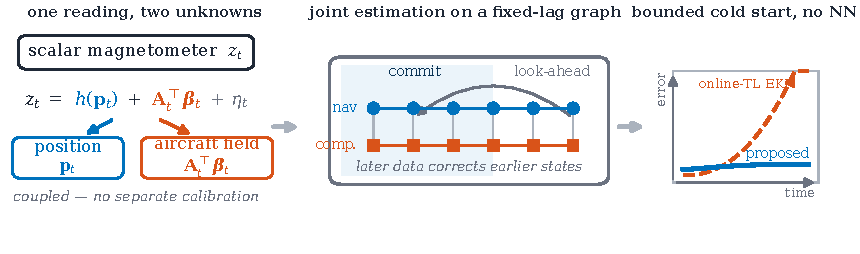
\includegraphics[width=0.98\textwidth]{figs/fig_concept.pdf}
\caption{Concept: one scalar reading couples position and compensation; a joint fixed-lag factor graph estimates both, emitting a causal and a smoothed answer.}
\label{fig:concept}
\end{figure*}

% P2a: Maturity of the field, and the two distinct deployment obstacles
Magnetic-anomaly navigation (MagNav) estimates aircraft position by matching the
measured scalar field against a surveyed anomaly map, yielding an absolute fix that
bounds inertial drift~\cite{canciani2017}. The idea has matured from feasibility
study to flight demonstration: recursive Bayesian map matching, from the extended
Kalman filter to grid and particle estimators, was characterized on flight
data~\cite{canciani2016,canciani2017} and flown on an F-16~\cite{canciani2020}, and
recent multi-hour fixed-wing trials over thousands of kilometres report
metre-to-decametre accuracy with quantum magnetometers~\cite{qctrl2025}. As the
estimators have matured, attention has moved to the inputs they rely on, and a
consensus is forming that the pacing requirement for operational deployment is a
sufficiently accurate, uncertainty-aware anomaly map~\cite{angappan2026}. Two
obstacles, in fact, separate these demonstrations from routine use, and they are
distinct: the reference map on the ground and the aircraft's own field in the air.
The map is a survey-and-data problem, pursued elsewhere~\cite{angappan2026}; this
paper addresses the second.

% P2b: The aircraft-field compensation problem
The platform's own permanent and induced magnetization and its eddy-current fields
perturb the scalar measurement by hundreds of nanotesla, comparable to or larger
than the anomaly signal being matched, so the aircraft field must be compensated
before map matching can recover position. This aircraft-field problem is intrinsic
to MagNav and independent of any particular airframe; it is most acute for
magnetometers mounted inside the cabin, close to avionics and current-carrying
structure, rather than on a wingtip stinger boom that holds the sensor away from the
platform field.

% P3: Technical Background -- two orthogonal difficulties, mostly attacked offline
Aeromagnetic compensation is classically handled by the Tolles--Lawson (TL)
model~\cite{tolles1950,leliak1961,bickel1979}, a regression of the interference onto
sixteen attitude-dependent terms (permanent, induced, and eddy-current) formed from a
three-axis fluxgate magnetometer. It faces two difficulties that are easy to conflate
but are in fact orthogonal. The first is temporal: the coefficients are
conventionally identified on a dedicated high-altitude calibration flight of
prescribed maneuvers, yet many operational scenarios admit none, and the coefficients
drift with temperature and configuration. In this cold-start regime they must be
estimated online and jointly with navigation, from the same measurements that fix
position, a coupling that makes both estimation and its analysis substantially harder
than the calibrated case. The second is representational: however well its
coefficients are fit, the linear TL basis cannot span interference from platform
currents and other non-rigid, non-attitude sources, which contribute a large fraction
of the field on cabin-mounted sensors~\cite{gnadt2020,gnadt2022}. One difficulty is
about identifying a known model class in time; the other is about that class being
too small.

A public benchmark has made both concrete: the Signal Enhancement for Magnetic
Navigation (SGL~2020) challenge dataset~\cite{gnadt2020}, with flight-grade INS,
wingtip-stinger and cabin-mounted magnetometers, and high-resolution anomaly maps.
Most work on it attacks the two difficulties offline: the TL coefficients by a
batch calibration flight, and the representational gap by learned models fit offline
on logged data, neural-network heading-error and denoising
compensators~\cite{williams1993,gnadt2022}, physics-informed liquid-time-constant
networks~\cite{nerrise2024}, and model-stability studies of the regression in
gradiometry~\cite{noriega2015}. Offline learning, however, presupposes exactly
what the operational scenario lacks: a corpus of logged flights from the same
aircraft, a reference-grade compensated sensor flying alongside to supply training
targets, the computation to train on that corpus, and a willingness to retrain
whenever the platform configuration or its magnetic state drifts. A compensator
fit this way is specific to one airframe in one equipment state, and its accuracy
in flight is bounded by how well the training corpus transfers to the day's
conditions. We therefore treat the offline family as context rather than
competition: every estimator compared in this paper starts, as ours does, from no
prior flight data. The exception is the online NN-in-EKF line of work
originated by Gnadt~\cite{gnadt2022}, which carries the TL coefficients and the
weights of a residual network as filter states learned in flight, and which has
recently been extended with an error-state formulation and a natural-gradient
interpretation~\cite{hager2026}; this lineage holds, to our knowledge, the
strongest reported cold-start results on the benchmark. This paper takes on the
temporal difficulty fully: online, joint estimation of a time-varying
compensation. The representational gap it does not model term-by-term: instead of a
learned remainder, the estimator absorbs what the TL basis misses structurally,
through the time-varying coefficients, a colored disturbance state, and a robust
kernel, and Section~\ref{sec:results} verifies against the recorded platform
currents how much of the remainder this accounts for.

% P4: Cluster A -- Bayesian filtering / map matching
Recursive Bayesian filtering is the standard machinery for map-matching
navigation, from the linear Kalman filter~\cite{kalman1960} to nonlinear variants.
Geophysical map matching has a long lineage: terrain-contour matching for cruise
missiles~\cite{golden1980} and nonlinear Kalman filtering for terrain-aided
navigation~\cite{hostetler1983} established the paradigm, and grid- and
particle-based Bayesian estimators later became standard where the
measurement-to-position map is strongly nonlinear or
multimodal~\cite{bergman1999,gustafsson2002,anonsen2006,nordlund2009}. For MagNav
specifically, Canciani and Raquet combined a calibrated scalar magnetometer with an
extended Kalman filter (EKF) and characterized the achievable accuracy on flight
data~\cite{canciani2016,canciani2017}, later demonstrating airborne magnetic
navigation with online calibration~\cite{canciani2020}. Beyond the EKF, unscented
filtering~\cite{julier2004}, invariant formulations that respect the state
manifold~\cite{barrau2017}, and mixture/particle representations~\cite{barshalom2001}
improve consistency under nonlinearity. However, these estimators are causal:
they commit each state online with no access to future measurements, and the
position-centric ones carry no compensation state of their own. When a large
uncompensated cold-start residual enters, a causal filter has no mechanism to
attribute the mismatch to the aircraft field rather than to position, and, unable to
revise a state once made, the estimate can diverge.

% P5: Cluster B -- online / learned compensation
A second line of work makes the compensation itself adaptive. Classical
Tolles--Lawson (TL) identification is a batch regression on a calibration
flight~\cite{tolles1950,leliak1961,bickel1979}; to remove that requirement the TL
regression can be embedded in the estimator and its coefficients tracked online as
additional states. Nonlinear extensions replace or augment the linear basis with
learned components: neural-network compensators date back three
decades~\cite{williams1993}, model-stability and robustness of the regression have
been studied in gradiometry~\cite{noriega2015}, and machine-learning-enhanced
calibration has recently been applied to the SGL benchmark~\cite{gnadt2022}. Most
relevant here, a residual neural network (NN) has been added on top of an online TL
model, carried inside an EKF and trained online, to capture interference the linear
basis misses, introduced with Gnadt's online models~\cite{gnadt2022} and recently
extended in~\cite{hager2026}; this reaches good cold-start accuracy on the SGL~2020
cabin magnetometers and holds, to our knowledge, the strongest reported cold-start
results on that benchmark. Nevertheless, the network requires a carefully
engineered online-training design to remain stable, adds opaque parameters whose
behavior is hard to certify, and, being embedded in an EKF, inherits the same
causal, commit-online limitation as the filters above.

% P6: Cluster C -- factor-graph smoothing
A third body of work, largely from robotics, replaces filtering with factor-graph
optimization: the estimation problem is a graph of variables and probabilistic
constraints~\cite{kschischang2001} whose maximum-a-posteriori (MAP) solution is
found by sparse nonlinear least squares~\cite{dellaert2017,dellaert2012}, the same
structure underlying bundle adjustment and graph SLAM~\cite{triggs2000,grisetti2010,kummerle2011}.
Incremental and square-root smoothers (square-root
SAM~\cite{dellaert2006}, iSAM~\cite{kaess2008}, iSAM2~\cite{kaess2012}, and
exactly-sparse delayed-state filters~\cite{eustice2006}) make the solution
efficient enough for online use, and fixed-lag sliding-window
optimization~\cite{sibley2010,leutenegger2015} bounds its cost. On-manifold inertial
preintegration~\cite{forster2017}, factor-graph inertial
fusion~\cite{indelman2013}, and modern visual--inertial estimators~\cite{qin2018}
have brought the approach firmly into navigation. Despite these advances,
factor-graph estimation in navigation has been developed almost entirely for
visual--inertial odometry and simultaneous localization and mapping, where the
estimated quantities are poses and landmarks. The factor graph has very recently
reached aeromagnetic compensation itself: Lathrop et al.~\cite{lathrop2024}
calibrate a magnetometer by fusing vector and scalar magnetometers with inertial
measurements in a factor graph, absorbing large permanent moments and a
time-varying external field. That work compensates the sensor but does not close
the loop to navigation. The joint problem, estimating a time-varying compensation
together with aircraft position from map matching, has not, to our knowledge, been
posed in a published factor-graph formulation, and the observability of doing so has
not been characterized.

% P6.5: Synthesis of the gap
Taken together, the three lines leave a specific gap. The cold-start MagNav problem
is fundamentally a joint estimation of position and a time-varying
compensation model from a single scalar stream, in which the two unknowns are
confounded through the very measurement that must resolve them. Causal filters
(cluster~A) must commit each state before the maneuvers that would disambiguate the
compensation have occurred, and so diverge when the initial residual is large;
learned online compensation (cluster~B) repairs that residual but keeps the causal,
commit-online architecture and adds parameters that are difficult to certify; and
factor-graph smoothing (cluster~C), which can defer commitment and estimate
structured nuisance variables jointly, has not been applied to this problem, nor has
anyone characterized when the joint problem is even observable. What is missing is
an estimator that (i)~defers commitment so that late-arriving calibration
information corrects early navigation states, (ii)~represents the compensation as
first-class, time-varying variables rather than a black box, and (iii)~comes with
an explicit condition for when position and compensation can be separated at all.
This paper supplies all three.

% P7: Proposed approach + contributions
In this work we cast cold-start magnetic-anomaly navigation as a factor graph
and, within it, carry the online Tolles--Lawson coefficients as time-varying
variables, so that navigation and compensation are solved jointly as one
maximum-a-posteriori (MAP) problem (Fig.~\ref{fig:concept}). The graph is
solved in real time by an incremental fixed-lag smoother built on
iSAM2~\cite{kaess2012}: states are placed at \SI{1}{\hertz}, variables older
than a \SI{300}{\second} lag are marginalized, and each update touches only the
part of the factorization the new measurement disturbs. Every state inside the
lag is relinearized and revised as later measurements arrive, so late
calibration information corrects early navigation states, the mechanism a
causal filter lacks; a causal filter commits each state once and cannot revise
it. We are explicit about scope: for a linear--Gaussian model the fixed-lag MAP
estimate coincides with classical fixed-lag smoothing~\cite{rauch1965}, so
smoothing per se is not the contribution; the joint estimation of a
time-varying compensation, delivered incrementally in real time, is.
The paper makes the following contributions:
\begin{enumerate}
  \item \textbf{Joint navigation and compensation on a factor graph.} We carry
        the online Tolles--Lawson coefficients as time-varying variables of a
        factor graph so that navigation and compensation are estimated jointly
        from the same scalar measurements. To the authors' knowledge this is
        the first factor-graph formulation that jointly estimates time-varying
        Tolles--Lawson compensation and navigation states at a calibration cold
        start. Relinearizing the coefficients as the graph is re-solved makes
        the compensation adapt along the flight, the role a learned online
        model plays in the competing filter, while the graph keeps every
        quantity an explicit, physically interpretable state.
  \item \textbf{A real-time incremental realization.} The graph is solved by an
        incremental fixed-lag smoother whose per-epoch cost is set by the lag,
        not the flight: \SIrange{7.3}{9.0}{\milli\second} per state at a
        \SI{300}{\second} lag and \SI{1}{\hertz} states, two orders of
        magnitude within the state cadence, in an unoptimized implementation.
        The lag is the principal architecture-level design variable, and we measure what it buys: the
        smoothed estimate improves steeply up to a knee near
        \SI{300}{\second}, about \SI{20}{\kilo\meter} of track, while the
        causal estimate is indifferent to it.
  \item \textbf{A causal/smoothed evaluation protocol.} A fixed-lag smoother
        produces two estimates, a causal one at the newest state and a
        smoothed one revised by the full lag, and comparisons in the
        literature rarely distinguish them. We report both throughout, so the
        comparison against causal filters is like for like and the price of
        latency is explicit: the causal output alone beats the recursive
        baselines on most cases, and the smoothed output roughly halves its
        error at the cost of lagging real time by the lag.
  \item \textbf{Flight-data validation.} On uncompensated cabin magnetometers
        across eight cold-start cases spanning four lines, two flights, two
        maps and two altitude regimes, under one untuned configuration, the
        smoothed estimate is the most accurate of the compared estimators on
        all eight cases and the causal estimate on six. Run rather than merely
        cited, the online EKF+TL+NN lineage of~\cite{gnadt2022,hager2026} is
        kept bounded by its network where a plain online-TL EKF diverges, yet
        the smoother beats it with no learned component; an ablation over
        every element of the configuration finds metre-level sensitivity and
        no delicate setting.
\end{enumerate}

% P8: Organization
The remainder of this paper is organized as follows.
Section~\ref{sec:problem} states the problem in its classical batch form and
formalizes the cold start. Section~\ref{sec:fgo} sets out factor graph
optimization from first principles. Section~\ref{sec:method} develops the joint
system model, its factor graph, and the incremental fixed-lag solution.
Section~\ref{sec:results} describes the protocol and baselines and reports the
experiments. Section~\ref{sec:conclusion} concludes.

\section{Problem Formulation}\label{sec:problem}
This section states what magnetic-anomaly navigation asks for in its classical
batch form, shows why the aircraft's own field prevents that form from being
answered directly, and states the problem solved in the rest of the paper.

\subsection{Batch map matching}\label{sec:batchmm}
Database-referenced navigation determines position by comparing a measured
profile against a stored map. Let $\mathbf{p}_{0:k}$ be the horizontal positions
of the aircraft over $k+1$ epochs, $z_{0:k}$ the scalar readings, and
$h(\cdot)$ the map lookup returning the field predicted at a position. The
classical batch estimate minimizes a profile-matching criterion, in mean
absolute or mean squared form,
\begin{equation}
J_{\mathrm{MAD}}=\frac{1}{k}\sum_{i=0}^{k}\big|\,z_i-h(\mathbf{p}_i)\big|,
\quad
J_{\mathrm{MSD}}=\frac{1}{k}\sum_{i=0}^{k}\big(z_i-h(\mathbf{p}_i)\big)^{2},
\label{eq:mad}
\end{equation}
subject to the inertial navigation system supplying the increments between
consecutive positions,
\begin{equation}
\mathbf{p}_i-\mathbf{p}_{i-1}=\Delta\mathbf{p}^{\mathrm{ins}}_i,
\qquad i=1,\dots,k,
\label{eq:inshard}
\end{equation}
so that the search is over a rigid profile translated by the single unknown
initial state,
\begin{equation}
\hat{\mathbf{p}}_{0:k}=\arg\min_{\mathbf{p}_{0:k}} J .
\label{eq:batchmm}
\end{equation}
Terrain-referenced navigation is solved in this form
routinely~\cite{hollowell1990,cowie2008}, and the same form underlies the
magnetic case~\cite{canciani2016,canciani2017}.

We state Eqs.~\eqref{eq:mad}--Eq.~\eqref{eq:batchmm} as the reference formulation of
database-referenced navigation rather than as a competing method: airborne
magnetic-anomaly navigation is in practice run recursively, with a Kalman filter
or a particle filter aiding the inertial
solution~\cite{canciani2017,gnadt2022}, and those are the baselines compared
against in Section~\ref{sec:results}. The batch form is worth writing down
because it makes two things explicit that the recursive implementations leave
implicit, and both matter here. It shows what the map contributes, namely the
agreement between a measured profile and a stored one. And it treats the
inertial increment as the hard constraint Eq.~\eqref{eq:inshard}, which is the
assumption the factor graph of Section~\ref{sec:fgo} relaxes by admitting the
increment as one more piece of uncertain information.

What Eq.~\eqref{eq:mad} presumes is that the residual $z_i-h(\mathbf{p}_i)$ is small
and unstructured once the position is right. For a scalar magnetometer mounted
on an aircraft this is false, and by a wide margin. The measurement carries the
aircraft's own magnetic field, generated by permanent magnetization, by
currents induced in the airframe, and by eddy currents, all of which depend on
the aircraft attitude in the Earth field and therefore change continuously along
a line. On the four flight lines used in Section~\ref{sec:results} the map value
along the flown track varies with a standard deviation of
\SIrange{123}{327}{\nano\tesla} and a peak-to-peak swing of
\SIrange{586}{2377}{\nano\tesla}: that variation is the entire position signal.
Against it, the uncompensated field at a cabin-mounted magnetometer is
\SIrange{1729}{1978}{\nano\tesla} root-mean-square over the first
\SI{300}{\second} of flight. The interference is not a perturbation of the
signal, it is larger than the signal's full range, and Fig.~\ref{fig:signal}
shows the two side by side over the representative line.

\begin{figure}[t]
\centering
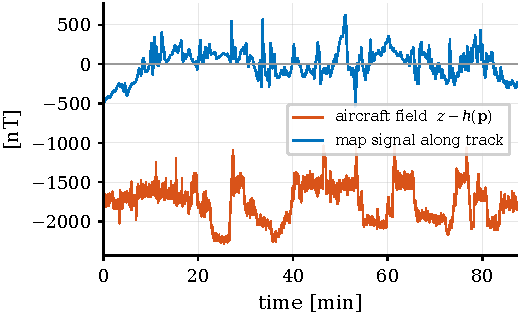
\includegraphics[width=\columnwidth]{figs/fig_signal.pdf}
\caption{Line 1007.06 Mag~4: the uncompensated aircraft field exceeds the full range of the map signal along the track.}
\label{fig:signal}
\end{figure}

Compensation is therefore not a refinement but a precondition. The classical
remedy is a calibration flight: a dedicated sequence of maneuvers at high
altitude, where the anomaly field is weak, from which the interference model is
fit once and then subtracted for the rest of the
mission~\cite{tolles1950,leliak1961,bickel1979}. That remedy is unavailable in
the situation this paper addresses. An aircraft that departs with an
uncalibrated installation, or whose interference has changed since its last
calibration, has no compensated measurement to feed
into Eq.~\eqref{eq:mad}. Estimating position then requires estimating the
compensation at the same time, from the same scalar stream that the map
matching consumes, and the two are coupled through that single stream: an error
in the compensation is indistinguishable, epoch by epoch, from an error in
position. We refer to this situation as a cold start, and it is the setting of
this paper.

\subsection{Problem statement}\label{sec:statement}
The situation just described fixes what has to be estimated and what may be
assumed. The aircraft carries a strapdown inertial navigation system whose
error grows without bound, a three-axis fluxgate, and a scalar magnetometer
whose reading is corrupted by the aircraft field. A gridded anomaly map of the
overflown region is available. No calibration flight has been made, so no
compensation model is known at takeoff, and no satellite navigation is
available at any point.

Formally, the problem this paper solves is the following:
given the scalar magnetometer measurements $z_{0:N}$, the fluxgate regressor
rows $\mathbf{A}_{0:N}$, the anomaly map $h$, the inertial mechanization, and a
prior $(\hat{\boldsymbol{\chi}}_0,\mathbf{P}_0)$ that assumes no prior
knowledge of the aircraft field, estimate the joint trajectory
$\boldsymbol{\chi}_{0:N}$ of inertial navigation errors $\mathbf{x}_k$ and
time-varying compensation coefficients $\boldsymbol{\beta}_k$, with a per-epoch
cost that does not grow with flight duration, so that the estimate is
available in flight.

Three properties of this problem shape the rest of the paper. It is
\emph{joint}, because the compensation cannot be measured separately from the
position it corrupts. It is \emph{underdetermined at any single epoch}, because
one scalar reading cannot separate a position error from a compensation error,
so the two are told apart only over a span of epochs. And it is
\emph{online}, because an estimator that must see the whole flight before
answering is of no use to the aircraft that flew it. The first two properties
call for an estimator that carries the compensation as a state and revises past
states as later data arrive; the third bounds how far into the past it may keep
revising. Sections~\ref{sec:fgo} and~\ref{sec:method} construct such an
estimator.

\section{Factor Graph Optimization}\label{sec:fgo}
The joint problem of Section~\ref{sec:statement} is stated as maximum a posteriori (MAP) inference and
solved on a factor graph. This section sets out that machinery from the
beginning, since the structure of the graph is what allows the compensation to
be carried as a first-class unknown and the estimate to be produced in real
time.

\subsection{Variables, factors, and the graph}
An estimation problem consists of quantities that are unknown and pieces of
information that constrain them. In a factor graph the two are drawn as two
kinds of node~\cite{loeliger2004,dellaert2017}. A \emph{variable node} holds an
unknown, here the state $\boldsymbol{\chi}_k$ at one epoch. A \emph{factor node}
holds one piece of information, and an edge joins a factor to every variable
that piece of information involves. No edge joins two variables or two factors,
so the graph is bipartite, and a factor is a function only of the variables it
touches. Fig.~\ref{fig:graph} shows this pattern for the graph this paper
builds in Section~\ref{sec:method}.

Three kinds of factor appear in any navigation graph, and they exhaust the ones
used in this paper. A \emph{prior} factor is unary and states what is believed
about a variable before any data: it fixes the otherwise free origin of the
estimate. A \emph{process} factor is binary and states how consecutive states are
related through the system dynamics and the inertial increments. A
\emph{measurement} factor is unary and states what a sensor reading predicts
about the state it was taken at. Writing $\mathbf{X}=\boldsymbol{\chi}_{0:N}$
for the collection of variables and $\mathbf{Z}$ for the data, the posterior
factors along exactly these edges,
\begin{equation}
p(\mathbf{X}\mid\mathbf{Z})\;\propto\;
p(\boldsymbol{\chi}_0)
\prod_{k=1}^{N}p(\boldsymbol{\chi}_k\mid\boldsymbol{\chi}_{k-1})
\prod_{k=0}^{N}p(z_k\mid\boldsymbol{\chi}_k),
\label{eq:posterior}
\end{equation}
which is written compactly as a product of factors
\begin{equation}
J(\mathbf{X};\mathbf{Z})=\prod_i\phi_i(\mathbf{X}_i;\mathbf{Z}),
\qquad
\hat{\mathbf{X}}=\arg\max_{\mathbf{X}}J(\mathbf{X};\mathbf{Z}),
\label{eq:prodfactors}
\end{equation}
with $\mathbf{X}_i$ the variables adjacent to factor $i$. The graph is a
picture of this factorization, and its sparsity is the problem's sparsity: each
factor constrains one or two states, never the whole trajectory at once.


\subsection{From factors to least squares}
Each factor is modelled with a Gaussian kernel about its predicted value,
\begin{equation}
\phi_i(\mathbf{X}_i;\mathbf{Z})\propto
\exp\!\Big(-\tfrac{1}{2}\big\lVert g_i(\mathbf{X}_i)-\mathbf{z}_i\big\rVert^{2}_{\mathbf{P}_i}\Big),
\label{eq:kernel}
\end{equation}
where $g_i$ is the prediction associated with the datum $\mathbf{z}_i$,
$\mathbf{P}_i$ its covariance, and
$\lVert\mathbf{e}\rVert_{\mathbf{P}}=\sqrt{\mathbf{e}^{\top}\mathbf{P}^{-1}\mathbf{e}}$
the Mahalanobis norm. Taking the negative logarithm of Eq.~\eqref{eq:prodfactors}
turns the product into a sum and the maximization into a nonlinear least-squares
problem,
\begin{equation}
\hat{\mathbf{X}}=\arg\min_{\mathbf{X}}\sum_i
\big\lVert g_i(\mathbf{X}_i)-\mathbf{z}_i\big\rVert^{2}_{\mathbf{P}_i}.
\label{eq:nlls}
\end{equation}
The Mahalanobis weighting is what makes this sum meaningful. Inertial
increments, magnetic readings in nanotesla, and compensation coefficients have
different units and differ in magnitude by orders; they become comparable only
after each residual is divided by its own uncertainty. The covariance attached
to a factor is therefore not bookkeeping, it sets how much authority that piece
of information carries against every other; Section~\ref{sec:coldprior} sets the
one covariance a cold start is sensitive to.

\subsection{Solving the graph}
Because $g_i$ is nonlinear in the states, Eq.~\eqref{eq:nlls} is solved
iteratively. Linearizing every residual about the current estimate
$\mathbf{X}^{(j)}$ and stacking gives
\begin{equation}
r(\mathbf{X})=
\begin{bmatrix} g_1(\mathbf{X}_1)-\mathbf{z}_1\\ \vdots\\
g_{N_f}(\mathbf{X}_{N_f})-\mathbf{z}_{N_f}\end{bmatrix},
\qquad
\mathcal{G}=\frac{\partial r}{\partial\mathbf{X}},
\label{eq:resstack}
\end{equation}
after which the Levenberg--Marquardt step
\begin{equation}
\Delta\mathbf{X}=-\big(\mathcal{G}^{\top}\mathcal{G}+\lambda\mathbf{I}\big)^{-1}
\mathcal{G}^{\top}r(\mathbf{X})
\label{eq:lm}
\end{equation}
is applied and the residuals are relinearized. The damping $\lambda$ interpolates
between Gauss--Newton and gradient descent and makes the iteration robust where
the problem is ill conditioned~\cite{dellaert2006}, which matters here because
the map term is strongly nonlinear.

Two consequences follow, and they are the reason for preferring this formulation
over a recursive filter. First, $\mathcal{G}$ inherits the sparsity of the graph:
a chain of process factors with unary measurements gives a block-bidiagonal
$\mathcal{G}$, so Eq.~\eqref{eq:lm} costs time linear in the number of states rather
than cubic. Second, every state is revised at every iteration. A filter commits
each state once, at the moment it is reached, and can never revisit it; the graph
relinearizes the whole set, so information that arrives late still corrects
estimates made early. In the cold start of Section~\ref{sec:batchmm} this is
exactly what is needed, because the compensation that explains the early
measurements is only identified after the aircraft has manoeuvred.

\subsection{Batch, fixed-lag, and incremental}
The formulation says nothing about how much of the flight $\mathbf{X}$ contains,
and that choice is the practical design variable. Taking $\mathbf{X}$ to be the
whole line gives the batch estimate: it uses every measurement and is the most
accurate, but it grows without bound and is available only after landing.
Restricting $\mathbf{X}$ to the states inside a bounded interval of the present,
and \emph{marginalizing} those that fall outside, gives a fixed-lag smoother
whose per-epoch cost does not grow with flight
duration~\cite{indelman2013,kaess2012}. Marginalization is not free: eliminating
a variable replaces its factors by a single dense factor on its former
neighbours, so what leaves the interval is summarized rather than discarded, and
it can no longer be revised.

Rebuilding and re-solving that interval from scratch at every epoch would waste
most of the work, since one new measurement changes little of a long chain.
Incremental solvers instead update the factorization in place, touching only the
part of it that the new data affect~\cite{kaess2012}. This is what makes a
fixed-lag smoother run at sensor rate, and it is the solver this paper uses;
Section~\ref{sec:incremental} states the construction and
Section~\ref{sec:lagdesign} measures what the length of the interval costs and
buys.

\section{Methodology}\label{sec:method}
Section~\ref{sec:batchmm} left the cold start with two unknowns coupled through
one scalar stream, and Section~\ref{sec:fgo} supplied a formulation in which
several unknowns of different kinds can be estimated together. This section puts
them together: the system model first, then the factor graph it induces, then
the incremental fixed-lag solution that produces an estimate in flight.

\subsection{System model}\label{sec:sysmodel}
The estimated quantity at epoch $k$ is the joint state
\begin{equation}
\boldsymbol{\chi}_k=\begin{bmatrix}\mathbf{x}_k\\ \boldsymbol{\beta}_k\end{bmatrix}
\in\mathbb{R}^{18+m},
\label{eq:jointstate}
\end{equation}
stacking the inertial error state $\mathbf{x}_k$ and the compensation
coefficients $\boldsymbol{\beta}_k$.

\subsubsection{Inertial error state}
We adopt the standard Pinson error model of a strapdown
INS~\cite{groves2013,titterton2004,farrell2008}. The error state
\begin{equation}
\mathbf{x}=\big[\,\delta\mathbf{p}^{\top}\;\delta\mathbf{v}^{\top}\;
\boldsymbol{\psi}^{\top}\;h_a\;\hat{a}\;\mathbf{b}_a^{\top}\;\mathbf{b}_g^{\top}\;S\,\big]^{\top}
\in\mathbb{R}^{18}
\label{eq:state}
\end{equation}
stacks position error $\delta\mathbf{p}$, velocity error $\delta\mathbf{v}$ and
attitude error $\boldsymbol{\psi}$ (three components each), the baro-inertial
altitude-aiding pair $(h_a,\hat{a})$ that damps the vertically unstable channel,
accelerometer and gyroscope biases $\mathbf{b}_a,\mathbf{b}_g$, and a scalar
first-order Gauss--Markov (FOGM) state $S$ that absorbs residual magnetic
disturbance and map error. Its discretized dynamics are
\begin{equation}
\mathbf{x}_{k}=\boldsymbol{\Phi}_{k-1}\mathbf{x}_{k-1}+\mathbf{w}_{k-1},
\qquad \mathbf{w}_{k-1}\sim\mathcal{N}(\mathbf{0},\mathbf{Q}_{k-1}),
\label{eq:dyn}
\end{equation}
with $\boldsymbol{\Phi}_{k}$ the Pinson state-transition matrix
(Appendix~\ref{app:pinson}) evaluated on the INS-indicated trajectory, and
$\mathbf{Q}_{k}$ the process covariance. Unlike the hard
constraint Eq.~\eqref{eq:inshard} of the batch form, the inertial increment enters
as a factor with a covariance, so the estimator may disagree with the INS in
proportion to how much that increment is trusted.

\subsubsection{Compensation state}
Classical aeromagnetic compensation writes the aircraft field as a linear
combination of attitude-dependent basis
terms~\cite{tolles1950,leliak1961,bickel1979},
\begin{equation}
c_k=\mathbf{A}_k^{\top}\boldsymbol{\beta}_k .
\label{eq:tl}
\end{equation}
With direction cosines $\hat{\mathbf{b}}_k=[\,u\;v\;w\,]^{\top}$ of the Earth
field in body axes, measured by a three-axis fluxgate, and total field magnitude
$B_k$, the permanent (3), induced (6) and eddy-current (9) groups are
\begin{equation}
\mathbf{A}_k=\big[\underbrace{u,v,w}_{\text{perm.}},\;
\underbrace{B_ku^2,\dots,B_kw^2}_{\text{induced}},\;
\underbrace{B_ku\dot u,\dots,B_kw\dot w}_{\text{eddy}}\big]^{\top},
\label{eq:tlbasis}
\end{equation}
optionally augmented by a constant term, giving $m\le19$ coefficients.
In the calibrated setting $\boldsymbol{\beta}$ is fit once on a calibration
flight and frozen. At a cold start it is unknown at takeoff, and the
installation state drifts slowly in flight, so we carry it as a variable with a
random-walk model
\begin{equation}
\boldsymbol{\beta}_{k}=\boldsymbol{\beta}_{k-1}+\mathbf{w}^{\beta}_{k-1},
\qquad \mathbf{w}^{\beta}_{k-1}\sim\mathcal{N}(\mathbf{0},\mathbf{Q}^{\beta}).
\label{eq:betawalk}
\end{equation}
This is the same device by which~\cite{park2023,park2024} carry slowly varying
sensor biases in a terrain-referenced graph. The difference is dimensional: a
radar-altimeter bias is one scalar, whereas Eq.~\eqref{eq:tlbasis} is an
$m$-dimensional regression whose columns are driven by aircraft attitude and
therefore excited only by manoeuvre.

\subsubsection{Measurement}
The scalar magnetometer reads
\begin{equation}
z_k=h(\mathbf{p}_k)+\mathbf{A}_k^{\top}\boldsymbol{\beta}_k+S_k+\eta_k,
\qquad \eta_k\sim\mathcal{N}(0,R),
\label{eq:meas}
\end{equation}
where $h(\cdot)$ interpolates the crustal anomaly map with the core field
restored, evaluated at the true position
$\mathbf{p}_k=\bar{\mathbf{p}}_k+\delta\mathbf{p}_k$ formed from the
INS-indicated position and the estimated position error. Linearizing the map
term about the INS-indicated position,
\begin{equation}
z_k\approx h(\bar{\mathbf{p}}_k)+\mathbf{g}_k^{\top}\delta\mathbf{p}_k
+\mathbf{A}_k^{\top}\boldsymbol{\beta}_k+S_k+\eta_k,
\qquad
\mathbf{g}_k=\left.\frac{\partial h}{\partial\mathbf{p}}\right|_{\bar{\mathbf{p}}_k},
\label{eq:measlin}
\end{equation}
which exposes the structure of the problem. The map gradient $\mathbf{g}_k$ is
the only channel through which the scalar reading carries horizontal position:
where the map is locally flat, $\mathbf{g}_k\!\approx\!\mathbf{0}$ and position
is momentarily unobservable. Everywhere else, the two terms
$\mathbf{g}_k^{\top}\delta\mathbf{p}_k$ and
$\mathbf{A}_k^{\top}\boldsymbol{\beta}_k$ compete for the same scalar: any
position error can be mimicked by a compensation error whose regressor
contribution matches it at that epoch. Separating them is possible only over a
span of epochs, because $\mathbf{g}_k$ follows the map under the flight path
while $\mathbf{A}_k$ follows the aircraft attitude, and the two vary
differently. This is the reason a smoother is used rather than a filter, and it
is quantified in Section~\ref{sec:obs}.

\subsection{Separability of position and compensation}\label{sec:obs}
The competition just described can be made exact. Collect, over a window of $W$
epochs, the horizontal position sensitivities (the vertical channel is
baro-aided) and the regressor rows of the linearized measurement
Eq.~\eqref{eq:measlin} into
\begin{equation}
\mathbf{G}=\begin{bmatrix}\mathbf{g}_1^{\top}\\ \vdots\\ \mathbf{g}_W^{\top}\end{bmatrix}
\in\mathbb{R}^{W\times2},
\qquad
\boldsymbol{\Psi}=\begin{bmatrix}\mathbf{A}_1^{\top}\\ \vdots\\ \mathbf{A}_W^{\top}\end{bmatrix}
\in\mathbb{R}^{W\times m},
\label{eq:gpsi}
\end{equation}
so that a constant position perturbation $\delta\mathbf{p}$ and a constant
coefficient perturbation $\delta\boldsymbol{\beta}$ change the residual
sequence by $\mathbf{G}\,\delta\mathbf{p}$ and
$\boldsymbol{\Psi}\,\delta\boldsymbol{\beta}$ respectively.

\begin{proposition}[Position separability]\label{prop:obs}
A position perturbation $\delta\mathbf{p}\neq\mathbf{0}$ is distinguishable
from every compensation adjustment over the window if and only if
$\mathbf{G}\,\delta\mathbf{p}\notin\mathrm{range}(\boldsymbol{\Psi})$.
Consequently every nonzero $\delta\mathbf{p}$ is distinguishable, so that the
pair $(\delta\mathbf{p},\delta\boldsymbol{\beta})$ is locally identifiable up
to $\delta\boldsymbol{\beta}\in\ker\boldsymbol{\Psi}$, and in particular
horizontal position is locally identifiable, if and only if
\begin{equation}
\operatorname{rank}\!\big[(\mathbf{I}-\boldsymbol{\Psi}\boldsymbol{\Psi}^{\dagger})\,\mathbf{G}\big]=2,
\label{eq:projrank}
\end{equation}
where $\dagger$ denotes the Moore--Penrose pseudoinverse.
\end{proposition}

The proof is in Appendix~\ref{app:proof}. The condition deliberately does not
ask for identifiability of $\boldsymbol{\beta}$ itself, which would require
$\ker\boldsymbol{\Psi}=\{\mathbf{0}\}$, because the \num{19}-term basis does
not satisfy it: in continuous time
$B_k(u\dot{u}+v\dot{v}+w\dot{w})=0$ ties the three diagonal eddy columns
exactly, and $B_k(u^2+v^2+w^2)=B_k$ makes the sum of the three diagonal
induced columns proportional to the constant bias column up to the variation
of the total field, about one percent RMS over a line. Both ties hold
exactly only in continuous time and are blurred at a comparable level by the
finite-differenced fluxgate rates; on the data they survive, since with every
column normalized to unit norm the smallest singular value of a
\SI{300}{\second} window of $\boldsymbol{\Psi}$ is still six orders of
magnitude below the largest. Navigation, however, needs the compensation
signal $\boldsymbol{\Psi}\boldsymbol{\beta}$, not the coefficients: two
coefficient vectors differing by an element of $\ker\boldsymbol{\Psi}$
produce the same correction, so the gauge is harmless to position, and
Eq.~\eqref{eq:projrank} is the condition that matters. The pseudoinverse
makes the condition gauge-invariant by construction, the projector onto
$\mathrm{range}(\boldsymbol{\Psi})$ being unchanged by the near-null
directions; numerically, the metric below moves by nothing across four
decades of rank tolerance. The FOGM disturbance $S_k$ of
Eq.~\eqref{eq:measlin} competes for the same scalar as well: its
window-constant part lies in $\mathrm{range}(\boldsymbol{\Psi})$ through the
bias column and is projected out with it, while its variation inside the
window is neglected in this analysis.

The condition also reads directly onto the estimator design. At a single
epoch, $\mathbf{G}$ has one row and the projected matrix has rank at most one,
so Eq.~\eqref{eq:projrank} can never hold: a memoryless correction cannot
separate the two effects. As the window grows, the map gradient under the
flight path and the attitude-driven regressor decorrelate and the projected
gradient accumulates rank and strength; the smallest eigenvalue of the Gram
matrix of the whitened projected gradient (the squared smallest singular
value),
\begin{equation}
\mu(W)=\lambda_{\min}\!\Big(\bar{\mathbf{G}}^{\top}
(\mathbf{I}-\bar{\boldsymbol{\Psi}}\bar{\boldsymbol{\Psi}}^{\dagger})
\bar{\mathbf{G}}\Big),
\label{eq:mu}
\end{equation}
with $\bar{\mathbf{G}}=R^{-1/2}\mathbf{G}$ and
$\bar{\boldsymbol{\Psi}}=R^{-1/2}\boldsymbol{\Psi}$ the noise-whitened
matrices, is a computable, flight-dependent measure of that strength:
$\mu(W)^{-1/2}$ is the weakest-direction position standard deviation that a
single isolated window of $W$ epochs supports under a static-coefficient
reading of the model. It is not a bound on the estimator's error, and its
assumptions cut both ways. It is optimistic in holding $\delta\mathbf{p}$
and $\boldsymbol{\beta}$ fixed across the window and the residual white; it
is pessimistic in seeing one window in isolation, whereas the smoother
carries information across windows through the marginal prior of
Eq.~\eqref{eq:schur} and the coefficients are quasi-static far beyond one
window. Its absolute level scales as $\sqrt{R}$, an assumed constant, and it
measures one direction while DRMS is a two-axis RMS. What survives these
caveats is the shape in $W$ and the comparison across lines, and
Section~\ref{sec:lagdesign} uses it for exactly that: where the knee sits,
and which line is weakest. The empirical ablation of
Section~\ref{sec:ablation} measures what the walk $\mathbf{Q}^{\beta}$, the
inertial process factors, and the priors add.

\begin{remark}\label{rem:floor}
The condition is geometric: it depends on the map gradient under the
flight path. Over a locally flat map, $\mathbf{G}\!\approx\!\mathbf{0}$,
the projected gradient of Eq.~\eqref{eq:projrank} loses rank and position
is unobservable regardless of the compensation: a map-information floor
that bounds every estimator.
\end{remark}

\subsection{Factor graph formulation}\label{sec:graphform}
The models of Section~\ref{sec:sysmodel} induce four factor types on the
variables $\boldsymbol{\chi}_{0:N}$, drawn in Fig.~\ref{fig:graph}. Following the
convention of Eq.~\eqref{eq:kernel}, each is written as a squared Mahalanobis
residual.

\begin{figure*}[t]
\centering
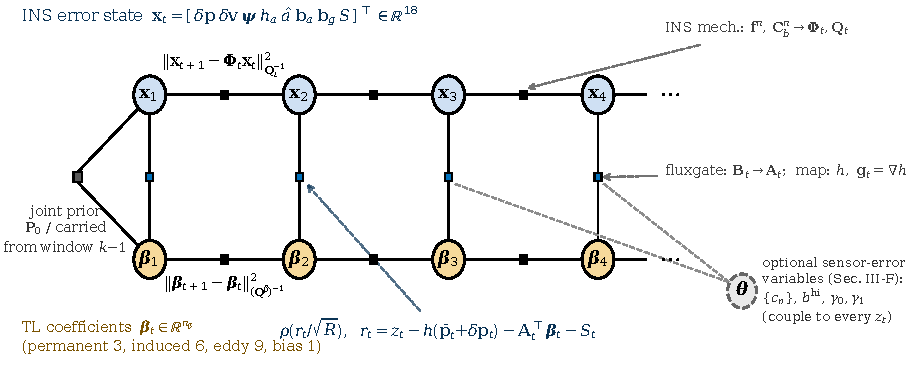
\includegraphics[width=0.96\textwidth]{figs/fig_graph.pdf}
\caption{Factor graph maintained by the smoother: two chains coupled at every epoch by the robust map factor carrying $z_k$; the marginal prior summarizes states older than the lag. Relief height is anomaly strength.}
\label{fig:graph}
\end{figure*}

The \emph{prior} factor anchors the initial joint state,
\begin{equation}
\bar{\phi}^{\,0}(\boldsymbol{\chi}_0)=
\big\lVert\boldsymbol{\chi}_0-\hat{\boldsymbol{\chi}}_0\big\rVert^{2}_{\mathbf{P}_0},
\label{eq:fprior}
\end{equation}
where $\mathbf{P}_0$ is block diagonal in the inertial and compensation parts,
with blocks $\mathbf{P}_0^{x}$ and $\mathbf{P}_0^{\beta}$.

The \emph{inertial} factor relates consecutive states through Eq.~\eqref{eq:dyn},
\begin{equation}
\bar{\phi}^{\,\mathrm{ins}}_k(\boldsymbol{\chi}_{k-1},\boldsymbol{\chi}_k)=
\big\lVert\mathbf{x}_k-\boldsymbol{\Phi}_{k-1}\mathbf{x}_{k-1}\big\rVert^{2}_{\mathbf{Q}_{k-1}} .
\label{eq:fins}
\end{equation}

The \emph{compensation} factor imposes the random walk Eq.~\eqref{eq:betawalk},
\begin{equation}
\bar{\phi}^{\,\beta}_k(\boldsymbol{\chi}_{k-1},\boldsymbol{\chi}_k)=
\big\lVert\boldsymbol{\beta}_k-\boldsymbol{\beta}_{k-1}\big\rVert^{2}_{\mathbf{Q}^{\beta}} ,
\label{eq:fbeta}
\end{equation}
so that the compensation is free to adapt along the flight at a rate set by
$\mathbf{Q}^{\beta}$, and is not free to jump.

The \emph{map} factor is the only one that couples the two chains,
\begin{equation}
\bar{\phi}^{\,\mathrm{map}}_k(\boldsymbol{\chi}_k)=
\rho\!\Big(\big\lVert h(\bar{\mathbf{p}}_k+\delta\mathbf{p}_k)
+\mathbf{A}_k^{\top}\boldsymbol{\beta}_k+S_k-z_k\big\rVert_{R}\Big),
\label{eq:fmap}
\end{equation}
with $\rho$ a robust kernel discussed below. Collecting the four types gives the
objective
\begin{equation}
\tilde{J}(\mathbf{X};\mathbf{Z})=\bar{\phi}^{\,0}(\boldsymbol{\chi}_0)
+\sum_{k=1}^{N}\bar{\phi}^{\,\mathrm{ins}}_k
+\sum_{k=1}^{N}\bar{\phi}^{\,\beta}_k
+\sum_{k=0}^{N}\bar{\phi}^{\,\mathrm{map}}_k ,
\label{eq:objective}
\end{equation}
minimized as in Eq.~\eqref{eq:nlls}. The graph has two parallel chains, the inertial
error and the compensation, tied together at every epoch by a map factor, and it
is this tie that makes the estimation joint rather than sequential.

Map error and transient interference produce heavy-tailed residuals that a
purely quadratic cost over-weights. We take $\rho$ to be the Huber
kernel~\cite{huber1964}
\begin{equation}
\rho(u)=\begin{cases}\tfrac12 u^2,& |u|\le\delta,\\
\delta\big(|u|-\tfrac12\delta\big),& |u|>\delta,\end{cases}
\label{eq:huber}
\end{equation}
minimized by iteratively reweighted least squares, in which each iteration
scales the map factor at epoch $k$ by $w_k=\min(1,\delta/|u_k|)$ with
$u_k=r_k/\sqrt{R}$, so that gross outliers are pulled toward an absolute-value
penalty while inliers keep the efficient quadratic cost. We use
$\delta=1.345$, the standard choice for $95\%$ Gaussian efficiency. Switchable
constraints~\cite{sunderhauf2012} and dynamic covariance
scaling~\cite{agarwal2013} fit the same factor interface and could
replace Eq.~\eqref{eq:huber} without touching the rest of the formulation.

\subsection{Incremental fixed-lag solution}\label{sec:incremental}
Minimizing Eq.~\eqref{eq:objective} over the whole line is a batch problem, and by
Section~\ref{sec:fgo} it is available only after the flight. For onboard use we
solve it at a fixed lag and incrementally.

\subsubsection{Fixed lag}
Let $L$ be the lag, in seconds. At epoch $k$ the graph retains the variables
whose timestamps lie within $L$ of the newest, and the variables older than that
are marginalized: their information is compressed into a Gaussian factor on the
oldest retained state, as described in Section~\ref{sec:fgo}. Two estimates are
therefore produced at every epoch, and they are different products.
\begin{itemize}
\item The \emph{causal} estimate is the value of the newest variable
$\boldsymbol{\chi}_k$ immediately after the update. It uses no measurement taken
after $k$, so it is available with zero delay and is the estimate that a
real-time navigator would read.
\item The \emph{smoothed} estimate is the value a variable holds when it
leaves the lag, after revision by every measurement in the following $L$
seconds: the classical fixed-lag smoothed output. It is the more accurate of
the two and it is available only $L$ seconds late.
\end{itemize}
Both are components of one optimization. Writing $J_k$ for the objective
Eq.~\eqref{eq:objective} restricted to the factors retained at epoch $k$,
together with the marginal prior of Eq.~\eqref{eq:schur} below, the smoother
computes the joint estimate and reads two components of it,
\begin{equation}
\hat{\mathbf{X}}_k=\arg\min_{\mathbf{X}}J_k(\mathbf{X}),\quad
\hat{\boldsymbol{\chi}}^{\mathrm{c}}_{k}=[\hat{\mathbf{X}}_k]_{k},\quad
\hat{\boldsymbol{\chi}}^{\mathrm{s}}_{k-\ell}=[\hat{\mathbf{X}}_k]_{k-\ell},
\label{eq:twoposteriors}
\end{equation}
with $\ell=L/\Delta$ the lag in states. Under a linear-Gaussian
specialization these components coincide with the classical filtering and
fixed-lag smoothing estimates, since a component of a Gaussian joint mode is
the corresponding marginal mean; in the nonlinear robust formulation they are
the current and delayed components of the fixed-lag joint MAP solution, and
any covariance attached to them is the Laplace approximation at the current
linearization and IRLS weights, without the M-estimator sandwich correction,
hence if anything optimistic.
Marginalization realizes the boundary compactly: if $\mathbf{x}_m$ denotes the
states leaving the lag and $\mathbf{x}_b$ the retained states their factors
touch, with joint information matrix and vector partitioned as
$\boldsymbol{\Lambda}=\big[\begin{smallmatrix}\boldsymbol{\Lambda}_{mm}&\boldsymbol{\Lambda}_{mb}\\
\boldsymbol{\Lambda}_{bm}&\boldsymbol{\Lambda}_{bb}\end{smallmatrix}\big]$,
$\boldsymbol{\eta}=\big[\begin{smallmatrix}\boldsymbol{\eta}_m\\
\boldsymbol{\eta}_b\end{smallmatrix}\big]$, then the marginal prior carried
forward is the Schur complement
\begin{equation}
\bar{\boldsymbol{\Lambda}}_{bb}
=\boldsymbol{\Lambda}_{bb}
-\boldsymbol{\Lambda}_{bm}\boldsymbol{\Lambda}_{mm}^{-1}\boldsymbol{\Lambda}_{mb},
\qquad
\bar{\boldsymbol{\eta}}_{b}
=\boldsymbol{\eta}_{b}
-\boldsymbol{\Lambda}_{bm}\boldsymbol{\Lambda}_{mm}^{-1}\boldsymbol{\eta}_{m},
\label{eq:schur}
\end{equation}
so for the linearized model no information is discarded. What is fixed is
the linearization at which Eq.~\eqref{eq:schur} is evaluated: for the
nonlinear factors the carried prior is a Laplace approximation, which can
inject slight overconfidence, an effect measured in
Section~\ref{sec:consistency}. This is the precise sense in which a smoothed
state can no longer be revised. Equation~\eqref{eq:schur} also requires
$\boldsymbol{\Lambda}_{mm}$ to be invertible, which the process-noise floor
of Section~\ref{sec:incremental} guarantees.

Both are reported throughout Section~\ref{sec:results}. Keeping them separate
matters for comparison: a causal filter such as an EKF can only be compared
against the causal estimate, whereas the smoothed estimate is the output of a
system that is allowed to lag real time by $L$.

\subsubsection{Incremental update}
Re-solving the retained interval from scratch at every epoch would repeat almost
all of the previous work, since one new measurement disturbs only a small part
of a long chain. We instead update the factorization in place using the
Bayes-tree formulation of iSAM2~\cite{kaess2012}. At each epoch the inertial
factor Eq.~\eqref{eq:fins}, the compensation factor Eq.~\eqref{eq:fbeta} and the map
factor Eq.~\eqref{eq:fmap} of that epoch are added; iSAM2 identifies the variables
whose linearization the new factors disturb, re-eliminates only that part of the
tree, and marginalizes what has left the lag. The per-epoch cost is therefore
set by the number of retained states, $L$ divided by the state interval, and not
by the flight duration.

\subsubsection{State interval}
Placing one variable per magnetometer sample makes the retained set large for
any useful lag. We therefore place variables at an interval $\Delta$ longer than
the sampling period, compounding the transition and accumulating the process
noise exactly across the $K$ samples that a variable interval spans,
\begin{equation}
\boldsymbol{\Phi}'=\boldsymbol{\Phi}_{k+K-1}\cdots\boldsymbol{\Phi}_{k},
\qquad
\mathbf{Q}'\leftarrow\boldsymbol{\Phi}\mathbf{Q}'\boldsymbol{\Phi}^{\top}+\mathbf{Q},
\label{eq:compound}
\end{equation}
so that the retained chain is an exact marginal of the full-rate chain in its
process model. The map factors at the intermediate samples are not carried:
at survey speed the along-track anomaly signal lies well below the
\SI{0.5}{\hertz} Nyquist frequency of the retained cadence, so the discarded
samples are largely redundant, and the cost of the choice is measured
directly in Section~\ref{sec:cost}.

\subsubsection{Conditioning}
One numerical point matters for reproduction. The position channel of
$\mathbf{Q}_k$ is minute, of order $10^{-31}\,\mathrm{rad}^2$ in the horizontal
states, because position error is driven only through velocity over a single
sample; whitening the inertial factor by $\mathbf{Q}_k^{-1/2}$ then spans some
thirty orders of magnitude. A Cholesky factorization of the information matrix
squares this conditioning and fails outright, returning an indeterminate
variable. Two changes remove the failure: a floor of $10^{-20}\mathbf{I}$ added
to $\mathbf{Q}_k$, which injects under a millimetre of position uncertainty per
step, and a QR factorization of the square-root
information matrix in place of Cholesky, which works on the square root and so
tolerates the residual spread~\cite{dellaert2006}. A larger floor, or a
regularizing prior at every epoch, also suppresses the exception but pins the
estimate onto the propagated INS and defeats the correction.

\subsection{Prior selection}\label{sec:coldprior}
One element of Eq.~\eqref{eq:fprior} is set with the cold start in mind. The block
$\mathbf{P}_0^{\beta}$ states what is believed about the compensation
coefficients before any measurement, and at a cold start that belief must admit
the field of an uncalibrated installation: the uncompensated cabin field is of
order \SI{2000}{\nano\tesla}, and the coefficients that explain it are far from
zero in the units of Eq.~\eqref{eq:tlbasis}. For initial stability we therefore
widen the compensation block relative to a calibrated installation and use
$\sigma_{\beta}=100$ throughout. The isotropic form mixes the units of the
coefficient groups; the dimensionally uniform alternative, a common prior
contribution of \SI{100}{\nano\tesla} per regressor column, performs
identically in the ablation. The setting is not delicate: the ablation of
Section~\ref{sec:ablation} varies it by an order of magnitude in each direction,
and every other element of the configuration, and finds metre-level effects.

\section{Experiments and Results}\label{sec:results}

\subsection{Dataset, maps, and protocol}\label{sec:protocol}

\begin{table}[t]
\caption{Flight lines (FF free flight, SV survey; maps R Renfrew, E Eastern) and free-inertial drift.}
\label{tab:lines}
\centering
\setlength{\tabcolsep}{4pt}
\begin{tabular}{llcccr}
\toprule
Line & Purp. & Map & alt.\ [m] & dur.\ [min] & INS [m] \\
\midrule
1003.02 & SV & E & 401 & 63.1 & 123.8 \\
1003.08 & SV & R & 400 & 72.4 & 271.9 \\
1007.02 & FF & E & 799 & 64.3 & 120.7 \\
1007.06 & FF & R & 402 & 87.3 & 317.5 \\
\bottomrule
\end{tabular}
\end{table}


\begin{table}[t]
\caption{Proposed-estimator settings, one configuration for every case.}
\label{tab:params}
\centering
\footnotesize
\setlength{\tabcolsep}{3pt}
\begin{tabular}{@{}llr@{}}
\toprule
Group & Parameter & Value \\
\midrule
Measurement & noise std.\ $\sqrt{R}$ & \SI{12}{\nano\tesla} \\
 & robust kernel, Huber $\delta$ & 1.345 \\
FOGM $S$ & $(\sigma_S,\tau)$ & \SI{3}{\nano\tesla}, \SI{180}{\second} \\
Initial $\mathbf{P}_0^{x}$ & pos.\ / alt.\ std. & \SI{0.1}{} / \SI{1.0}{\meter} \\
 & velocity std.\ (per axis) & \SI{1.0}{\meter\per\second} \\
Compensation & basis (App.~\ref{app:tl}) & P{+}I{+}E{+}bias ($m=19$) \\
 & prior $\mathbf{P}_0^{\beta}=\mathbf{I}\sigma_{\beta}^2$ & $\sigma_{\beta}=100$ \\
 & walk $\mathbf{Q}^{\beta}$ & $\mathbf{I}(1.0)^2\Delta t$ \\
Smoother & lag $L$ & \SI{300}{\second} \\
 & state interval $\Delta$ & \SI{1}{\second} ($K=10$) \\
 & solver & iSAM2, QR \\
 & process-noise floor & $10^{-20}\mathbf{I}$ \\
Evaluation & DRMS warm-up & \SI{600}{\second} \\
\bottomrule
\end{tabular}
\end{table}

All experiments use the public SGL~2020 challenge dataset~\cite{gnadt2020}: a
Cessna~208B instrumented with a flight-grade INS, several onboard scalar
magnetometers (a compensated tail-stinger sensor and uncompensated cabin sensors
Mag~4 and Mag~5, all optically pumped cesium-vapor units), a three-axis
fluxgate, and reference truth. The flights serve distinct purposes, and we
choose lines accordingly (Table~\ref{tab:lines}). Flt1007 is the free-flight
mission, in which the aircraft flies freely within the mapped areas, so its
lines are the closest to a navigation task and are what prior
work~\cite{gnadt2020,canciani2017,hager2026} reports; 1007.06 is our
representative line for that reason. Flt1003 is a crustal-field survey flight,
and its lines 1003.02 and 1003.08 are straighter than the free-flight legs.
Flt1006 is a calibration-manoeuvre flight and, with the map-building flights
(Flt1004--1005), is not used: its single \SI{14}{\minute} line leaves too little
to score after the warm-up.
Two honest points remain. None of these lines is a dedicated long,
straight-and-level operational transit; the free-flight and survey legs carry
attitude variation, which stresses the compensation but also aids its
observability by exciting the regressor, so performance on a pure operational
cruise is not established here. And the lines span two altitude regimes, four
near the \SI{400}{\meter} survey-drape altitude and 1007.02 near
\SI{800}{\meter}, where upward continuation attenuates the anomaly.

Map matching uses the Eastern and Renfrew high-resolution anomaly grids,
upward-continued to flight altitude, with the IGRF core field restored so that
measurement and map share an absolute scale. Cold start means the compensation
coefficients are initialized at zero with no calibration flight; the navigation
solution itself is accurately initialized (position standard deviation
\SI{0.1}{\meter}, Table~\ref{tab:params}), so the term denotes a compensation
cold start, not an unknown-position start.

The error metric is the horizontal distance root-mean-square (DRMS) of position
error, counted after a \SI{600}{\second} warm-up. Following
Section~\ref{sec:incremental}, the proposed estimator is reported twice in every
table: the \emph{causal} value, read at the newest state with no look-ahead,
and the \emph{smoothed} value, read as states leave the \SI{300}{\second} lag.
The causal value is the like-for-like comparison against the recursive
baselines, which also use no future data; the smoothed value is the output of
a system permitted to lag real time by the lag length, and the look-ahead
behind every reported number is stated in its table. One configuration
(Table~\ref{tab:params}) is used for every line and both magnetometers; nothing
is tuned per case, and parameter sensitivity is quantified in the ablation of
Section~\ref{sec:ablation}. All numbers are produced by scripted runs under a
fixed software environment and are available from the authors on request.

\subsection{Baselines}\label{sec:baselines}
Four references frame the comparison, all run by us on the same lines, the same
maps, and the same inertial model. Table~\ref{tab:params} describes the
proposed estimator; each baseline runs the configuration of its reference
implementation, including the compensation prior $\sigma_{\beta}=1$ of the
published EKF~\cite{gnadt2022}, and any departure from a published
configuration is stated below.

\emph{Free-inertial INS.} The unaided INS drift (Table~\ref{tab:lines}) is the
floor every aided estimator must beat, and the common reference that makes DRMS
values comparable across lines of different length and roughness.

\emph{Online-TL EKF.} The direct recursive counterpart of the proposed
estimator: the same Pinson error state augmented with the same \num{19}
time-varying TL coefficients, updated by the same scalar measurement, in an
extended Kalman filter~\cite{gnadt2022}. It shares every model term with the
factor graph, so the margin between the two isolates the estimator structure,
recursive commitment against windowed re-linearization, from the modelling.

\emph{Online EKF+TL+NN.} The strongest causal baseline we compare
against augments the TL state with the weights of a small feed-forward network
that absorbs what the linear basis cannot~\cite{gnadt2022,hager2026}. We run
the reference implementation of~\cite{gnadt2022}, tuned by us for a stable cold
start, and do not claim to reproduce the extended filter of~\cite{hager2026}.
Cold start forces one substantive change: with no calibration flight to
warm-start from, the network output normalization is initialized from the first
five minutes of onboard interference; a naive port instead drives the network
bias to $\sim\!5\times10^{4}$\,\si{\nano\tesla} and the filter to \texttt{NaN}.
We keep the uncompensated scalar out of the network inputs: a
position-dependent input carries the map gradient, so the network absorbs map
signal and position drifts while the residual stays small (the scalar-augmented
variant of~\cite{hager2026} escapes this only by freezing the network after its
transient). The tuned filter uses the permanent TL group with an eight-unit
hidden layer and reaches \num{48.8}/\SI{18.3}{\meter} on 1007.06 Mag~4/5,
consistent with published cold-start operating
points~\cite{gnadt2022,hager2026}.

\emph{Marginalized particle filter (MPF+TL).} The nonparametric reference,
included because particle methods are the standard resort when the map term is
strongly nonlinear~\cite{nordlund2009,park2024}. Since the TL model is linear
in its coefficients, $\boldsymbol{\beta}$ is conditionally linear-Gaussian and
fits the Rao--Blackwellized structure exactly: our implementation carries
position in \num{1000} particles and marginalizes the remaining states,
including $\boldsymbol{\beta}$, in the conditional Kalman block, with the
fluxgate row entering the linear measurement Jacobian. Weights are computed in
the log domain and position diversity is reinjected after resampling. The
filter's cold-start behaviour is dominated by the compensation prior. Run at
$\sigma_{\beta}=1$, the scale of a calibrated installation, it fails at
kilometre scale on every Mag~4 case: the conditional Kalman block then
predicts a measurement variance orders of magnitude below the truth, and the
particle weights degenerate into a directed walk up the local map gradient.
Matching the prior to the installation scale ($\sigma_{\beta}=700$, the
magnitude the fitted coefficients reach) repairs the dominant term, bringing
five of the eight cases to \SIrange{25}{95}{\meter} (\SI{1227}{} to
\SI{93.5}{\meter} on 1007.06 Mag~4), but both sensors of 1007.02, the line
with the weakest separability in Fig.~\ref{fig:obsmetric}, still diverge, and
the results remain seed-sensitive. The contrast with the windowed estimator
is the instructive part: a one-step filter must trust its compensation prior
at every epoch, whereas the smoother amortizes the same prior over the window
and is insensitive to it across two orders of magnitude
(Section~\ref{sec:ablation}). We therefore report the MPF in the text rather
than in the comparison tables, and we do not claim it represents the best
achievable particle filter.
Attaching the neural network of the EKF+TL+NN to the particle filter does not
rescue it and is sharply harmful on the well-conditioned sensor, degrading
Mag~5 by one to two orders of magnitude across lines, the same direction seen
for the NN-augmented EKF where the linear basis already suffices.

\subsection{Representative line}\label{sec:repline}

\begin{figure}[t]
\centering
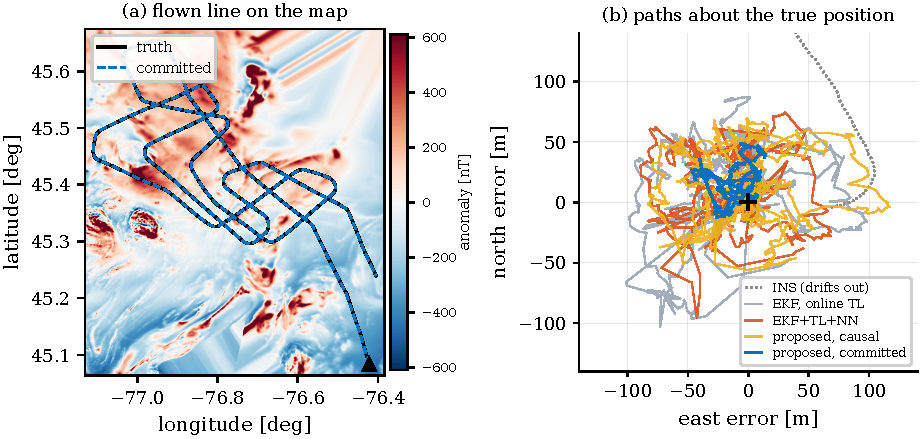
\includegraphics[width=\columnwidth]{figs/fig_track.pdf}
\caption{Line 1007.06 Mag~4: (a) flown line with the zoom window; (b) the estimated paths separate from the truth, at the largest post-warm-up EKF error.}
\label{fig:track}
\end{figure}


\begin{figure}[t]
\centering
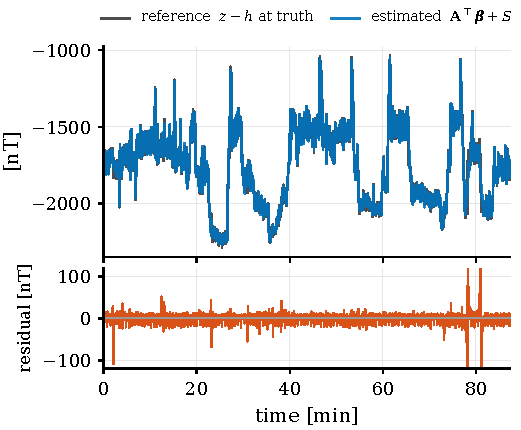
\includegraphics[width=\columnwidth]{figs/fig_comp.pdf}
\caption{Estimated $\mathbf{A}^{\top}\boldsymbol{\beta}+S$ against the interference reference, and the residual (line 1007.06 Mag~4).}
\label{fig:comp}
\end{figure}


\begin{table}[t]
\caption{Line 1007.06 cold start: DRMS [m] after a \SI{600}{\second} warm-up.}
\label{tab:1007}
\centering
\begin{tabular}{lrrc}
\toprule
Estimator & Mag 4 & Mag 5 & look-ahead \\
\midrule
EKF, online TL & 46.7 & 17.8 & none \\
EKF{+}TL{+}NN~\cite{gnadt2022} & 48.8 & 18.3 & none \\
\midrule
Proposed, causal & 42.7 & 16.0 & none \\
\textbf{Proposed, \SI{300}{\second} lag (smoothed)} & \textbf{24.2} & \textbf{11.5} & \SI{300}{\second} \\
\bottomrule
\end{tabular}
\end{table}

Table~\ref{tab:1007} reports the longest line, 1007.06 (\SI{87}{\minute}), on
both cabin magnetometers, with the free-inertial drift at \SI{317.5}{\meter}.
Read causally, with no look-ahead at all, the proposed estimator reaches
\SI{42.7}{\meter} on Mag~4 and \SI{16.0}{\meter} on Mag~5, ahead of the
online-TL EKF (\num{46.7}/\SI{17.8}{\meter}) and of the NN-augmented filter
(\num{48.8}/\SI{18.3}{\meter}). The margin over the online-TL EKF is the purest
number in this paper: the two estimators share the error model, the
compensation model, the measurement model, and every noise setting, and differ
only in that the filter commits each state once while the graph relinearizes
and revises every state inside its lag. The margin over the EKF+TL+NN says
something further: the network exists to absorb what the linear TL basis
cannot, yet carrying the linear basis in a smoother beats carrying the linear
basis plus a network in a filter, on both sensors, without any learned
component. Allowed its \SI{300}{\second} lag, the smoothed estimate roughly
halves the causal error, to \num{24.2}/\SI{11.5}{\meter}. Fig.~\ref{fig:errhist}
shows the error history, Fig.~\ref{fig:latlon} its north and east components
against every baseline, Fig.~\ref{fig:track} the recovered track on the map,
and Fig.~\ref{fig:comp} the compensation the graph learned while recovering it.

\begin{figure}[t]
\centering
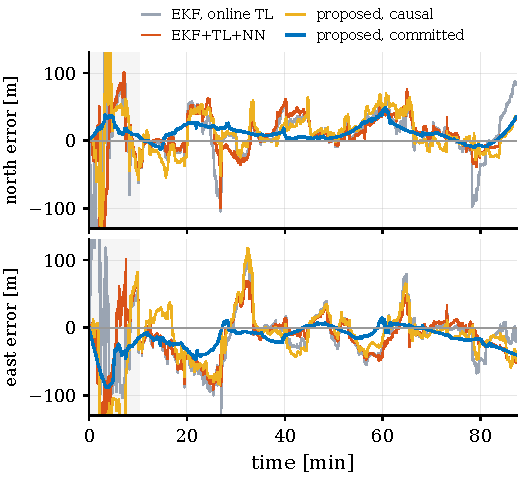
\includegraphics[width=\columnwidth]{figs/fig_latlon.pdf}
\caption{North and east error histories, line 1007.06 Mag~4. The seed-sensitive EKF+TL+NN is a fresh run (\SI{40.0}{\meter} here).}
\label{fig:latlon}
\end{figure}

\begin{figure}[t]
\centering
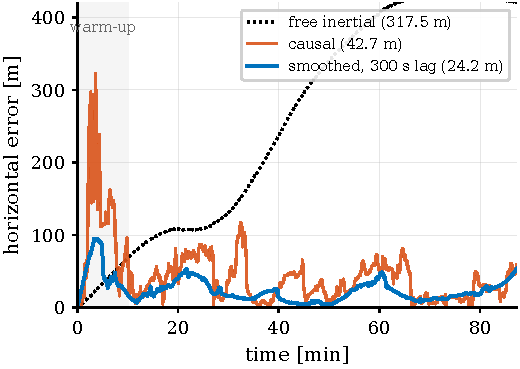
\includegraphics[width=\columnwidth]{figs/fig_errhist.pdf}
\caption{Horizontal error, line 1007.06 Mag~4: the smoothed trace is the causal trace revised by the \SI{300}{\second} lag.}
\label{fig:errhist}
\end{figure}

\subsection{Evaluation across lines and sensors}\label{sec:breadth}

\begin{figure}[t]
\centering
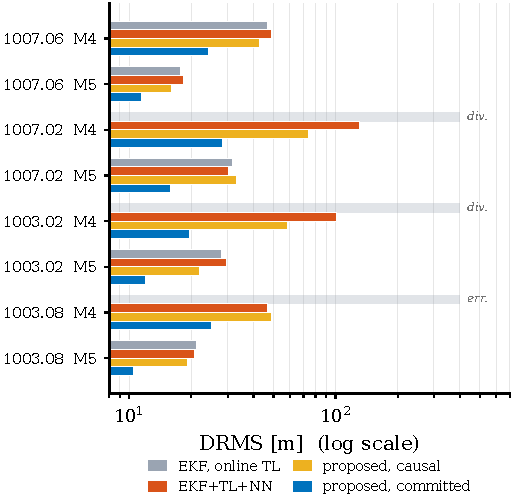
\includegraphics[width=\columnwidth]{figs/fig_breadthbar.pdf}
\caption{Breadth comparison of Table~\ref{tab:breadth}, log axis.}
\label{fig:breadthbar}
\end{figure}


\begin{table}[t]
\caption{Breadth: DRMS [m]. ``div.''\ $>\SI{10}{\kilo\meter}$, ``err.''\ leaves the map; bold = best overall.}
\label{tab:breadth}
\centering
\setlength{\tabcolsep}{3.5pt}
\begin{tabular}{llrr rr}
\toprule
 & & EKF & EKF{+} & \multicolumn{2}{c}{Proposed} \\
\cmidrule(l){5-6}
Line & Mag & online & TL{+}NN & causal & \SI{300}{\second} lag \\
\midrule
1007.06 & 4 & 46.7 & 48.8 & 42.7 & \textbf{24.2} \\
1007.06 & 5 & 17.8 & 18.3 & 16.0 & \textbf{11.5} \\
1007.02 & 4 & div. & 130.0 & 74.3 & \textbf{28.4} \\
1007.02 & 5 & 31.6 & 30.4 & 33.1 & \textbf{15.8} \\
1003.02 & 4 & div. & 101.0 & 58.2 & \textbf{19.6} \\
1003.02 & 5 & 28.1 & 29.5 & 21.9 & \textbf{12.0} \\
1003.08 & 4 & err. & 46.6 & 48.9 & \textbf{25.0} \\
1003.08 & 5 & 21.1 & 20.7 & 19.2 & \textbf{10.5} \\
\midrule
\multicolumn{4}{l}{best causal} & \textbf{6 / 8} & \\
\multicolumn{4}{l}{best overall} & & \textbf{8 / 8} \\
\bottomrule
\end{tabular}
\end{table}

Table~\ref{tab:breadth} repeats the comparison on every counted line, spanning
two flights, two maps, two altitude regimes, and both cabin magnetometers, with
nothing re-tuned (Fig.~\ref{fig:breadthbar}). The smoothed estimate is the most accurate entry on all
eight counted cases, between \SI{10.5}{} and \SI{28.4}{\meter}, and between
\num{1.5} and \num{5.2} times better than the strongest causal baseline on the
same case. Read causally, the proposed estimator is the best causal method on
six of the eight; it trails the EKF+TL+NN on 1007.02 Mag~5 by \SI{2.7}{\meter}
and on 1003.08 Mag~4 by \SI{2.3}{\meter}, and we report both rather than
claiming a sweep. Where the online-TL EKF fails outright, diverging on two
Mag~4 lines and leaving the map on a third, both readings of the proposed
estimator stay bounded; the mechanism is the one
Section~\ref{sec:sysmodel} anticipated, since the filter must explain the
uncompensated field with whatever state is cheapest at each instant, while the
smoother may revise its attribution for \SI{300}{\second} before committing.

\subsection{Lag design}\label{sec:lagdesign}

\begin{figure}[t]
\centering
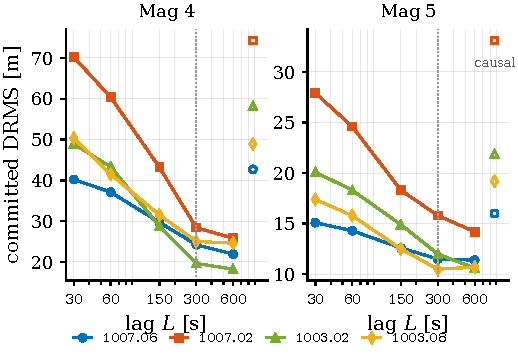
\includegraphics[width=\columnwidth]{figs/fig_lagsweep.pdf}
\caption{Smoothed DRMS against lag; open markers show the lag-independent causal error.}
\label{fig:lagsweep}
\end{figure}


\begin{table}[t]
\caption{Lag sweep: smoothed DRMS [m]; the causal output varies by under a metre across the sweep.}
\label{tab:lag}
\centering
\setlength{\tabcolsep}{4pt}
\begin{tabular}{ll rrrrr r}
\toprule
 & & \multicolumn{5}{c}{lag $L$ [s], smoothed} & causal \\
\cmidrule(lr){3-7}
Line & Mag & 30 & 60 & 150 & 300 & 600 & \\
\midrule
1007.06 & 4 & 40.2 & 37.1 & 29.7 & 24.2 & 21.9 & 42.7 \\
1007.06 & 5 & 15.1 & 14.3 & 12.6 & 11.5 & 11.4 & 16.0 \\
1007.02 & 4 & 70.2 & 60.4 & 43.2 & 28.4 & 25.8 & 74.3 \\
1007.02 & 5 & 27.9 & 24.6 & 18.3 & 15.8 & 14.2 & 33.1 \\
1003.02 & 4 & 48.9 & 43.3 & 28.8 & 19.6 & 18.2 & 58.2 \\
1003.02 & 5 & 20.1 & 18.3 & 14.9 & 12.0 & 10.6 & 21.9 \\
1003.08 & 4 & 50.3 & 41.5 & 31.5 & 25.0 & 24.6 & 48.9 \\
1003.08 & 5 & 17.4 & 15.8 & 12.5 & 10.5 & 10.7 & 19.2 \\
\bottomrule
\end{tabular}
\end{table}

\begin{figure}[t]
\centering
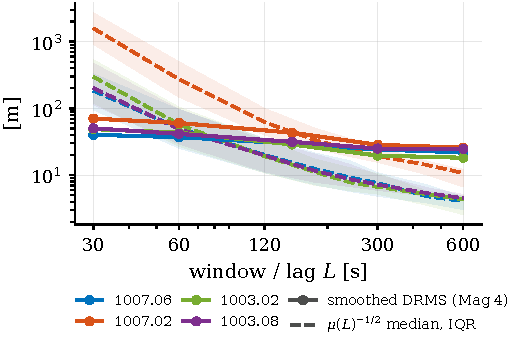
\includegraphics[width=\columnwidth]{figs/fig_obsmetric.pdf}
\caption{Separability metric $\mu^{-1/2}$ of Eq.~\eqref{eq:mu} at window
length $L$ (dashed, median and interquartile range over sliding windows)
against the measured smoothed DRMS at lag $L$ (solid, Mag~4; the metric is
sensor-independent), per line.}
\label{fig:obsmetric}
\end{figure}

The lag is the estimator's principal design variable, and Table~\ref{tab:lag}
sweeps it from \SI{30}{} to \SI{600}{\second} on the four counted lines (Fig.~\ref{fig:lagsweep}). Two
regularities carry the design guidance. First, the smoothed error improves
monotonically with lag up to \SI{300}{\second} on every case, and weakly
after it: lengthening the lag from \SI{300}{} to \SI{600}{\second}, a
doubling of both latency and computation, buys at most \SI{2.6}{\meter} and on
one case slightly degrades, while the step from \SI{30}{} to \SI{300}{\second}
buys between \SI{3.6}{} and \SI{41.8}{\meter}. The knee is anticipated by the
separability metric of Eq.~\eqref{eq:mu}: Fig.~\ref{fig:obsmetric} evaluates
$\mu^{-1/2}$ in sliding windows of length equal to the lag, at the
\SI{1}{\hertz} kept cadence. Being a single-window quantity, the metric does
not bound the smoothed error, which draws on information carried across
windows by the marginal prior: at \SI{30}{\second} the per-line medians are
\SIrange{184}{1585}{\meter} while the measured smoothed DRMS is
\SIrange{15.1}{70.2}{\meter}. It is also blind to the magnetometer, so the
Mag~4 to Mag~5 gap is outside its reach. What it carries is the shape and
the geography, and both match. The metric falls by one and a half to two
orders of magnitude between \SI{30}{} and \SI{300}{\second}, the range in
which the measured smoothing gain is concentrated; past \SI{300}{\second}
the measured DRMS stops improving even though the single-window metric keeps
falling, so beyond the knee the error is no longer separability-limited but
set by map error, inertial noise, and coefficient drift, which more
look-ahead does not remove. And the metric identifies the weakest line:
1007.02, lowest at every window length (median \SI{19.3}{\meter} at
\SI{300}{\second} against \SIrange{6.7}{7.6}{\meter} for the other three),
is the line with the largest measured error at every lag on both sensors.
We take \SI{300}{\second} as the default. Second, the causal column is flat: across a
twentyfold change in lag the causal error moves by less than a metre on every
case. The lag decides only how long a state is revised before it is frozen, not
how good the newest state is, so the accuracy bought by look-ahead is entirely
smoothing gain, and a designer who cannot afford latency loses exactly the gap
between the two columns and nothing else.

\subsection{Ablation}\label{sec:ablation}

\begin{table}[t]
\caption{Ablation on line 1007.06, one change per row: smoothed (causal) DRMS [m].}
\label{tab:ablation}
\centering
\setlength{\tabcolsep}{4pt}
\begin{tabular}{l l rr}
\toprule
Element & Change & Mag 4 & Mag 5 \\
\midrule
\multicolumn{2}{l}{reference ($\sigma_{\beta}=100$)} & 24.2 (42.7) & 11.5 (16.0) \\
\midrule
Comp.\ prior & $\sigma_{\beta}=10$ & 24.1 (43.9) & 11.5 (16.6) \\
 & $\sigma_{\beta}=1000$ & 23.9 (42.1) & 11.2 (15.4) \\
 & per column, \SI{100}{\nano\tesla} & 23.7 (42.7) & 11.6 (16.1) \\
Comp.\ walk & $\mathbf{Q}^{\beta}\times0.01$ & 26.3 (56.4) & 12.7 (20.0) \\
 & $\mathbf{Q}^{\beta}\times100$ & 24.1 (42.7) & 12.4 (25.8) \\
FOGM & $\sigma_S\times10$ & 23.9 (38.8) & 11.0 (16.6) \\
Robust kernel & removed & 25.4 (42.9) & 11.7 (16.5) \\
 & Huber $\delta=10$ & 25.6 (42.8) & 11.7 (16.5) \\
Meas.\ noise & $\sqrt{R}=\SI{65}{\nano\tesla}$ & 24.6 (42.9) & 12.7 (23.7) \\
Process floor & $10^{-16}\mathbf{I}$ & 33.1 (74.7) & 13.1 (19.3) \\
Relin. & every variable, every epoch & 24.1 (42.6) & 11.5 (16.0) \\
Meas.\ density & all \num{10} samples per state & 26.5 (44.2) & 11.7 (16.0) \\
\bottomrule
\end{tabular}
\end{table}

Table~\ref{tab:ablation} varies each element of the configuration on line
1007.06, one at a time. The estimator is insensitive at the metre level to all
of them. The compensation prior may move an order of magnitude in either
direction, or be replaced by a per-column prior that assigns each regressor
column \SI{100}{\nano\tesla} of measurement contribution, for changes under a
metre. Slowing the compensation walk a hundredfold costs about two metres,
consistent with a real installation state that drifts in flight; speeding it up
costs little. Removing the Huber kernel or widening its threshold costs one to
two metres, so robustness to map error helps but does not carry the result.
Inflating the assumed measurement noise fivefold, or relinearizing every
variable at every epoch, changes the estimate by less than half a metre; the
latter confirms that iSAM2's selective relinearization gives up nothing here.
The largest single effect is the process-noise floor: raising it from
$10^{-16}$ to $10^{-12}$ times the nominal position channel, i.e.\ from
$10^{-20}\mathbf{I}$ to $10^{-16}\mathbf{I}$, costs \SI{8.9}{\meter} on Mag~4,
which is why Section~\ref{sec:incremental} treats the floor as a conditioning
device to be kept minimal rather than a tuning knob. Attaching all ten raw
measurements to each state instead of one costs \SI{2.3}{\meter} on Mag~4 and
nothing on Mag~5, at four times the computation, supporting the
\SI{1}{\hertz} state cadence.

\subsection{Cold-start transient and initial uncertainty}\label{sec:transient}

\begin{table}[t]
\caption{First \SI{600}{\second} of the cold start: DRMS and peak horizontal
error [m] inside the warm-up window.}
\label{tab:transient}
\centering
\setlength{\tabcolsep}{4pt}
\begin{tabular}{ll rr rr}
\toprule
 & & \multicolumn{2}{c}{smoothed} & \multicolumn{2}{c}{causal} \\
\cmidrule(lr){3-4}\cmidrule(l){5-6}
Line & Mag & DRMS & peak & DRMS & peak \\
\midrule
1007.06 & 4 & 55.0 & 95.0 & 135.5 & 323.1 \\
1007.06 & 5 & 10.7 & 18.6 & 41.2 & 107.6 \\
1007.02 & 4 & 36.7 & 73.3 & 93.2 & 220.3 \\
1007.02 & 5 & 36.5 & 53.2 & 65.2 & 134.4 \\
1003.02 & 4 & 21.5 & 48.9 & 72.3 & 206.8 \\
1003.02 & 5 & 11.9 & 15.2 & 40.0 & 107.6 \\
1003.08 & 4 & 23.3 & 31.4 & 110.6 & 303.6 \\
1003.08 & 5 & 13.2 & 18.8 & 31.0 & 57.1 \\
\bottomrule
\end{tabular}
\end{table}

Every DRMS so far excludes the first \SI{600}{\second}, so Table~\ref{tab:transient}
reports what happens inside that window, when the compensation is least
known. The smoothed value of an epoch is the value it holds when it leaves
the lag, so every entry in the smoothed columns has been revised by up to
\SI{300}{\second} of later measurements. The estimator does not pass through
a divergent phase: the smoothed output runs at \SIrange{10.7}{55.0}{\meter}
DRMS during the transient, within \SI{30}{\percent} of its own converged
value on six of the eight cases and within a factor of \num{2.3} on the
remaining two. What the transient taxes is causality. The causal output
peaks between \SI{57}{} and \SI{323}{\meter}, and over the same interval the
free-inertial drift is only \SIrange{33}{65}{\meter} DRMS with peaks of
\SIrange{64}{116}{\meter}: while the window is too short for position and
compensation to be separable (Proposition~\ref{prop:obs} at small $W$), the
causal estimate can attribute interference to position in a way the unaided
INS cannot, and on most cases it is transiently worse than coasting. The
mis-attribution is repaid within the lag, since the smoothed revision of the
same epochs is already at the converged scale, and after the warm-up the
causal output beats the free-inertial drift on every counted case.

The cold start of this paper assumes a known takeoff position
(\SI{0.1}{\meter} horizontal prior) and an unknown installation field.
Relaxing the former tests how much the results lean on it: widening the
initial horizontal position prior to \SI{10}{}, \SI{50}{}, and
\SI{100}{\meter} on both sensors of 1007.06 moves the post-warm-up smoothed
DRMS by at most \SI{0.4}{\meter} (\SI{24.19}{} to \SI{24.54}{\meter} on
Mag~4, \SI{11.53}{} to \SI{11.66}{\meter} on Mag~5) and the causal DRMS by
at most \SI{4.6}{\meter}. The transient pays more: at the \SI{100}{\meter}
prior the in-window smoothed DRMS rises from \SI{55.0}{} to
\SI{69.1}{\meter} on Mag~4 and from \SI{10.7}{} to \SI{22.0}{\meter} on
Mag~5, while the causal transient is essentially unchanged. The two cases of
Table~\ref{tab:transient} that beat their converged values do so by leaning
on the tight anchor, and the advantage disappears with it. The information
that converges the estimator is the map gradient accumulated over the first
window, not the decimetre anchor, and the post-warm-up claims do not depend
on a surveyed takeoff point.

\subsection{Statistical consistency}\label{sec:consistency}
Whether the reported covariance can be believed is a separate question from
accuracy, and we answer it in two parts, formal and diagnostic.

\emph{Monte Carlo under a perfect model.} The error-state truth is simulated
from the estimator's own discretized model on the 1007.06 geometry, the
transition and process noise of Eq.~\eqref{eq:compound} at the \SI{1}{\hertz}
cadence, and measurements are synthesized from the same map, regressor, and
$R$ with Gaussian noise; the robust kernel is disabled, since the noise is
truly Gaussian, and the smoother runs exactly as flown otherwise. For each
epoch the two-degree-of-freedom horizontal-position NEES
$\mathbf{e}^{\top}\mathbf{P}^{-1}\mathbf{e}$ is evaluated with the marginal
covariance $\mathbf{P}$ from the Bayes tree, at the newest state for the
causal output and at the state leaving the lag for the smoothed output. The
synthetic measurements are generated through the nonlinear map at the
perturbed position, so linearization error is present in the experiment.
Over \num{20} independent runs the causal average NEES is $2.03\pm0.19$ and
the smoothed average $2.26\pm0.27$, mean and 95\% $t$-interval over run
means, against the consistent value of \num{2}; within-run samples are
serially correlated over the lag, so the run-level spread, not a per-sample
chi-square band, is the honest error bar. The causal output is statistically
consistent. The smoothed marginal is on average about \SI{13}{\percent} too
small in the NEES (variance) sense, \SI{6}{\percent} in standard deviation,
at the edge of significance, consistent with, though not isolated to, the
linearizations frozen at marginalization
(Section~\ref{sec:incremental}). The test exercises the Gaussian
specialization; the robust kernel of the flown configuration is outside its
scope.

\emph{Coverage in flight.} On real data the model is not perfect, the map
carries error and the interference is not white, so the same statistic is a
diagnostic of the reported covariance rather than a consistency test. On
1007.06, the fraction of post-warm-up epochs whose horizontal error lies
inside the 95\% ellipse of the reported Laplace covariance
($\chi^2_2$ threshold \num{5.99}) is \SI{93}{\percent} causal and
\SI{62}{\percent} smoothed on Mag~5, and \SI{53}{\percent} causal and
\SI{27}{\percent} smoothed on Mag~4; the errors are correlated over roughly
the lag, so these fractions carry an effective sample size of order tens,
not thousands. The pattern is informative: the covariance is nearly honest
where the model is nearly right, and optimistic exactly where unmodeled map
error and residual interference dominate, more so for the smoothed output
whose reported uncertainty is smaller. Restoring \SI{95}{\percent} coverage
would take a standard-deviation inflation of roughly \num{1.1} (Mag~5
causal) to \num{3} (Mag~4 smoothed); an integrity layer built on this
estimator should inflate accordingly, and the accuracy claims of this paper
rest on the measured DRMS, not on the reported covariance.

\subsection{Computational cost}\label{sec:cost}
All timings are single-core, on a laptop-class x86 processor under WSL2, with
the measurement factor evaluated through a Python callback; they are upper
bounds on a native implementation. At the reference configuration the
incremental update takes \SIrange{7.3}{9.0}{\milli\second} per state across the
eight counted line--magnetometer cases, mean \SI{8.2}{\milli\second},
so the
\SI{87}{\minute} line completes in \SI{42}{\second} and the margin to the
\SI{1}{\hertz} state cadence exceeds two orders of magnitude. The cost scales
with the number of retained states, so halving the lag halves it, and the two
expensive variants of the ablation bound the alternatives: relinearizing every
variable at every epoch costs \SI{68}{\milli\second} per state and attaching
all ten raw measurements \SI{31}{\milli\second}, both still real time at
\SI{1}{\hertz} but paying roughly ninefold and fourfold for accuracy changes
the ablation shows to be, respectively, below half a metre and a two-metre
degradation.

\section{Conclusion}\label{sec:conclusion}
This paper posed cold-start magnetic-anomaly navigation as a single estimation
problem: an aircraft with an uncalibrated magnetometer installation must
recover its position from a scalar reading in which the map signal and the
aircraft's own field are mixed, with no calibration flight and no satellite
aiding. The formulation carries the Tolles--Lawson compensation coefficients as
time-varying variables of a factor graph alongside the inertial error state,
ties the two chains through the map measurement, and solves the graph with an
incremental fixed-lag smoother built on iSAM2, at a \SI{300}{\second} lag and a
\SI{1}{\hertz} state cadence. The estimator produces two outputs, a causal
estimate with no look-ahead and a smoothed estimate revised by the full lag,
and we report both throughout, because they answer different questions: the
causal output is what a navigator reads in flight, the smoothed output is what
a system that may lag real time delivers.

On the SGL~2020 flight data the answers are as follows. Against a recursive EKF
carrying the identical models, the causal output alone is more accurate on six
of eight cold-start cases, so windowed relinearization pays before any
look-ahead is spent. Against an NN-augmented online EKF baseline, an EKF
augmented with an online neural network, the linear-basis smoother is more
accurate on both magnetometers of the representative line with no learned
component at all. The smoothed output is the most accurate estimate on all
eight counted cases, between \SI{10.5}{} and \SI{28.4}{\meter} where
free-inertial drift is hundreds of metres, at \num{1.5} to \num{5.2} times the
accuracy of the best causal baseline. The lag sweep locates the design knee
near \SI{300}{\second}, about \SI{20}{\kilo\meter} of track, and shows that the
causal output is indifferent to the lag, so the choice of lag is purely a
purchase of smoothing accuracy with latency. The ablation finds no delicate
setting: one configuration serves every line and both sensors, and the update
costs \SIrange{7.3}{9.0}{\milli\second} per state in an unoptimized
implementation, two orders of magnitude inside real time.

Several limitations bound the study. Each line is a single physical
realization, so every DRMS is a point estimate; the statistical statements are
counts across cases, not distributions. The reported covariance of the
incremental smoother has not been validated for consistency on flight data,
and we do not report uncertainty bounds. The
baselines are our own implementations under one shared protocol; the
particle-filter reference in particular is reported as unstable under per-case
tuning, and we do not claim it represents the best achievable particle filter.
None of the lines is a long, straight-and-level operational transit, so
performance under the weak regressor excitation of a pure cruise is not
established. And the compensation prior that a cold start needs is a measured
setting rather than a derived one: we show a broad insensitive range, but give
no rule for choosing its scale from installation data.

These limitations set the agenda: consistency evaluation of the reported
covariance, a transit-like flight regime, sparser instantiation of the
compensation chain in the manner of~\cite{park2024}, and a native-factor
implementation that would carry the real-time margin from the state cadence
down to the raw sensor rate.

\appendices
\section{Pinson Error-State Dynamics}\label{app:pinson}
The navigation-error block of $\boldsymbol{\Phi}_t$ in Eq.~\eqref{eq:dyn} follows the
Pinson model in a local north-east-down frame~\cite{titterton2004,groves2013}. With
position, velocity, and attitude errors $(\delta\mathbf{p},\delta\mathbf{v},
\boldsymbol{\psi})$ and sensor biases $(\mathbf{b}_a,\mathbf{b}_g)$, the continuous
error dynamics are
\begin{equation}
\begin{aligned}
\dot{\delta\mathbf{p}}&=\mathbf{F}_{pp}\,\delta\mathbf{p}+\delta\mathbf{v},\\
\dot{\delta\mathbf{v}}&=\mathbf{F}_{vp}\,\delta\mathbf{p}
+\mathbf{F}_{vv}\,\delta\mathbf{v}
-[\mathbf{f}^n\times]\,\boldsymbol{\psi}+\mathbf{C}^n_b\mathbf{b}_a,\\
\dot{\boldsymbol{\psi}}&=\mathbf{F}_{\psi p}\,\delta\mathbf{p}
+\mathbf{F}_{\psi v}\,\delta\mathbf{v}
-[\boldsymbol{\omega}^n_{in}\times]\,\boldsymbol{\psi}-\mathbf{C}^n_b\mathbf{b}_g,
\end{aligned}
\label{eq:pinson}
\end{equation}
where $\mathbf{f}^n$ is the specific force, $\mathbf{C}^n_b$ the body-to-nav rotation,
$\boldsymbol{\omega}^n_{in}$ the inertial rate, $[\cdot\times]$ the skew operator, and
the $\mathbf{F}_{\bullet\bullet}$ blocks collect the transport-rate, gravity-gradient,
and Coriolis terms. The biases follow first-order Gauss--Markov or random-walk models,
as does the scalar magnetic disturbance state $S$ with correlation time $\tau$. The
discrete $\boldsymbol{\Phi}_t=\exp(\mathbf{F}_t\,\Delta t)$ and $\mathbf{Q}_t$ are
obtained by standard van~Loan discretization~\cite{farrell2008}. Only
$\mathbf{g}_t^{\top}$, the position row of the linearized
measurement Eq.~\eqref{eq:measlin}, couples this block to the map.

\section{Tolles--Lawson Basis}\label{app:tl}
The basis row $\mathbf{A}_t$ of Eq.~\eqref{eq:tlbasis} is built from the fluxgate
direction cosines $\hat{\mathbf{b}}=[\,u\;v\;w\,]^{\top}$ (with $u^2+v^2+w^2=1$) and
the scalar field magnitude $B$~\cite{tolles1950,leliak1961}. The permanent moment
contributes the three cosines $(u,v,w)$; the induced magnetization, symmetric in the
field, contributes the six products
$B\,(u^2,uv,uw,v^2,vw,w^2)$; and the eddy-current field, proportional to the rate of
change of the cosines, contributes the nine products $B\,(u\dot u,u\dot v,\dots,
w\dot w)$. Stacking these gives an eighteen-term basis, optionally augmented by a
constant bias, and $c_t=\mathbf{A}_t^{\top}\boldsymbol{\beta}_t$ is linear in the
coefficients $\boldsymbol{\beta}_t$, the property that lets them enter the factor
graph as ordinary linear-measurement variables. In the cold-start regime the
calibration flight that classically fixes $\boldsymbol{\beta}$ is unavailable, which
is precisely why we carry it as a graph variable.

\section*{Acknowledgment}
The experiments use the publicly released SGL~2020 challenge
dataset~\cite{gnadt2020}.

\begin{biography}[{
\includegraphics[width=1in,height=1.25in,clip,keepaspectratio]{figs/author_lee.png}}]{Jayden Dongwoo Lee}
received the M.S. degree in aerospace engineering from the Korea Advanced Institute
of Science and Technology (KAIST), Daejeon, South Korea, in 2021. He is currently
pursuing the Ph.D. degree in aerospace engineering at KAIST. His research interests
include unmanned aircraft systems (UAS), guidance and navigation, adaptive and
data-driven control, and estimation.
\end{biography}

\begin{biography}[{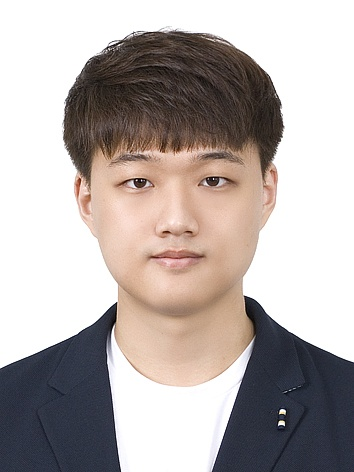
\includegraphics[width=1in,height=1.25in,clip,keepaspectratio]{figs/author_chang.png}}]{Bohyun Chang}
is with the Department of Aerospace Engineering, Korea Advanced Institute of Science
and Technology (KAIST), Daejeon, South Korea. His research interests include
guidance, navigation, and control of aerospace vehicles.
\end{biography}

\begin{biography}[{
\includegraphics[width=1in,height=1.25in,clip,keepaspectratio]{figs/author_bang.jpg}}]{Hyochoong Bang}
received his Ph.D. degree in aerospace engineering from Texas
A\&M University in 1992. Since 2001, he has been with the Department of Aerospace
Engineering, Korea Advanced Institute of Science and Technology (KAIST), Daejeon,
South Korea, as a professor. His research interests include spacecraft guidance,
attitude dynamics and control, unmanned aerial vehicle flight dynamics and control,
and flight control system design.
\end{biography}

\section{Proof of Proposition~\ref{prop:obs}}\label{app:proof}
Over the window, a position perturbation $\delta\mathbf{p}$ and a coefficient
perturbation $\delta\boldsymbol{\beta}$ change the stacked residual by
$\mathbf{G}\,\delta\mathbf{p}+\boldsymbol{\Psi}\,\delta\boldsymbol{\beta}$.
The perturbation $\delta\mathbf{p}$ is indistinguishable from a compensation
adjustment exactly when some $\delta\boldsymbol{\beta}$ cancels it, that is
when $\mathbf{G}\,\delta\mathbf{p}=-\boldsymbol{\Psi}\,\delta\boldsymbol{\beta}
\in\mathrm{range}(\boldsymbol{\Psi})$, which proves the first statement.
For the second, decompose
$\mathbf{G}\,\delta\mathbf{p}=\boldsymbol{\Psi}\boldsymbol{\Psi}^{\dagger}
\mathbf{G}\,\delta\mathbf{p}+(\mathbf{I}-\boldsymbol{\Psi}\boldsymbol{\Psi}^{\dagger})
\mathbf{G}\,\delta\mathbf{p}$: the first term always lies in
$\mathrm{range}(\boldsymbol{\Psi})$, so
$\mathbf{G}\,\delta\mathbf{p}\in\mathrm{range}(\boldsymbol{\Psi})$ if and only
if $(\mathbf{I}-\boldsymbol{\Psi}\boldsymbol{\Psi}^{\dagger})\mathbf{G}\,
\delta\mathbf{p}=\mathbf{0}$. Hence every nonzero $\delta\mathbf{p}$ is
distinguishable if and only if the projected matrix
$(\mathbf{I}-\boldsymbol{\Psi}\boldsymbol{\Psi}^{\dagger})\mathbf{G}$ has
trivial kernel, that is rank two. \hfill$\blacksquare$


\bibliographystyle{IEEEtaes}
\bibliography{references}

\end{document}
